\documentclass[1p]{elsarticle_modified}
%\bibliographystyle{elsarticle-num}

%\usepackage[colorlinks]{hyperref}
%\usepackage{abbrmath_seonhwa} %\Abb, \Ascr, \Acal ,\Abf, \Afrak
\usepackage{amsfonts}
\usepackage{amssymb}
\usepackage{amsmath}
\usepackage{amsthm}
\usepackage{scalefnt}
\usepackage{amsbsy}
\usepackage{kotex}
\usepackage{caption}
\usepackage{subfig}
\usepackage{color}
\usepackage{graphicx}
\usepackage{xcolor} %% white, black, red, green, blue, cyan, magenta, yellow
\usepackage{float}
\usepackage{setspace}
\usepackage{hyperref}

\usepackage{tikz}
\usetikzlibrary{arrows}

\usepackage{multirow}
\usepackage{array} % fixed length table
\usepackage{hhline}

%%%%%%%%%%%%%%%%%%%%%
\makeatletter
\renewcommand*\env@matrix[1][\arraystretch]{%
	\edef\arraystretch{#1}%
	\hskip -\arraycolsep
	\let\@ifnextchar\new@ifnextchar
	\array{*\c@MaxMatrixCols c}}
\makeatother %https://tex.stackexchange.com/questions/14071/how-can-i-increase-the-line-spacing-in-a-matrix
%%%%%%%%%%%%%%%

\usepackage[normalem]{ulem}

\newcommand{\msout}[1]{\ifmmode\text{\sout{\ensuremath{#1}}}\else\sout{#1}\fi}
%SOURCE: \msout is \stkout macro in https://tex.stackexchange.com/questions/20609/strikeout-in-math-mode

\newcommand{\cancel}[1]{
	\ifmmode
	{\color{red}\msout{#1}}
	\else
	{\color{red}\sout{#1}}
	\fi
}

\newcommand{\add}[1]{
	{\color{blue}\uwave{#1}}
}

\newcommand{\replace}[2]{
	\ifmmode
	{\color{red}\msout{#1}}{\color{blue}\uwave{#2}}
	\else
	{\color{red}\sout{#1}}{\color{blue}\uwave{#2}}
	\fi
}

\newcommand{\Sol}{\mathcal{S}} %segment
\newcommand{\D}{D} %diagram
\newcommand{\A}{\mathcal{A}} %arc


%%%%%%%%%%%%%%%%%%%%%%%%%%%%%5 test

\def\sl{\operatorname{\textup{SL}}(2,\Cbb)}
\def\psl{\operatorname{\textup{PSL}}(2,\Cbb)}
\def\quan{\mkern 1mu \triangleright \mkern 1mu}

\theoremstyle{definition}
\newtheorem{thm}{Theorem}[section]
\newtheorem{prop}[thm]{Proposition}
\newtheorem{lem}[thm]{Lemma}
\newtheorem{ques}[thm]{Question}
\newtheorem{cor}[thm]{Corollary}
\newtheorem{defn}[thm]{Definition}
\newtheorem{exam}[thm]{Example}
\newtheorem{rmk}[thm]{Remark}
\newtheorem{alg}[thm]{Algorithm}

\newcommand{\I}{\sqrt{-1}}
\begin{document}

%\begin{frontmatter}
%
%\title{Boundary parabolic representations of knots up to 8 crossings}
%
%%% Group authors per affiliation:
%\author{Yunhi Cho} 
%\address{Department of Mathematics, University of Seoul, Seoul, Korea}
%\ead{yhcho@uos.ac.kr}
%
%
%\author{Seonhwa Kim} %\fnref{s_kim}}
%\address{Center for Geometry and Physics, Institute for Basic Science, Pohang, 37673, Korea}
%\ead{ryeona17@ibs.re.kr}
%
%\author{Hyuk Kim}
%\address{Department of Mathematical Sciences, Seoul National University, Seoul 08826, Korea}
%\ead{hyukkim@snu.ac.kr}
%
%\author{Seokbeom Yoon}
%\address{Department of Mathematical Sciences, Seoul National University, Seoul, 08826,  Korea}
%\ead{sbyoon15@snu.ac.kr}
%
%\begin{abstract}
%We find all boundary parabolic representation of knots up to 8 crossings.
%
%\end{abstract}
%\begin{keyword}
%    \MSC[2010] 57M25 
%\end{keyword}
%
%\end{frontmatter}

%\linenumbers
%\tableofcontents
%
\newcommand\colored[1]{\textcolor{white}{\rule[-0.35ex]{0.8em}{1.4ex}}\kern-0.8em\color{red} #1}%
%\newcommand\colored[1]{\textcolor{white}{ #1}\kern-2.17ex	\textcolor{white}{ #1}\kern-1.81ex	\textcolor{white}{ #1}\kern-2.15ex\color{red}#1	}

{\Large $\underline{12a_{0935}~(K12a_{0935})}$}

\setlength{\tabcolsep}{10pt}
\renewcommand{\arraystretch}{1.6}
\vspace{1cm}\begin{tabular}{m{100pt}>{\centering\arraybackslash}m{274pt}}
\multirow{5}{120pt}{
	\centering
	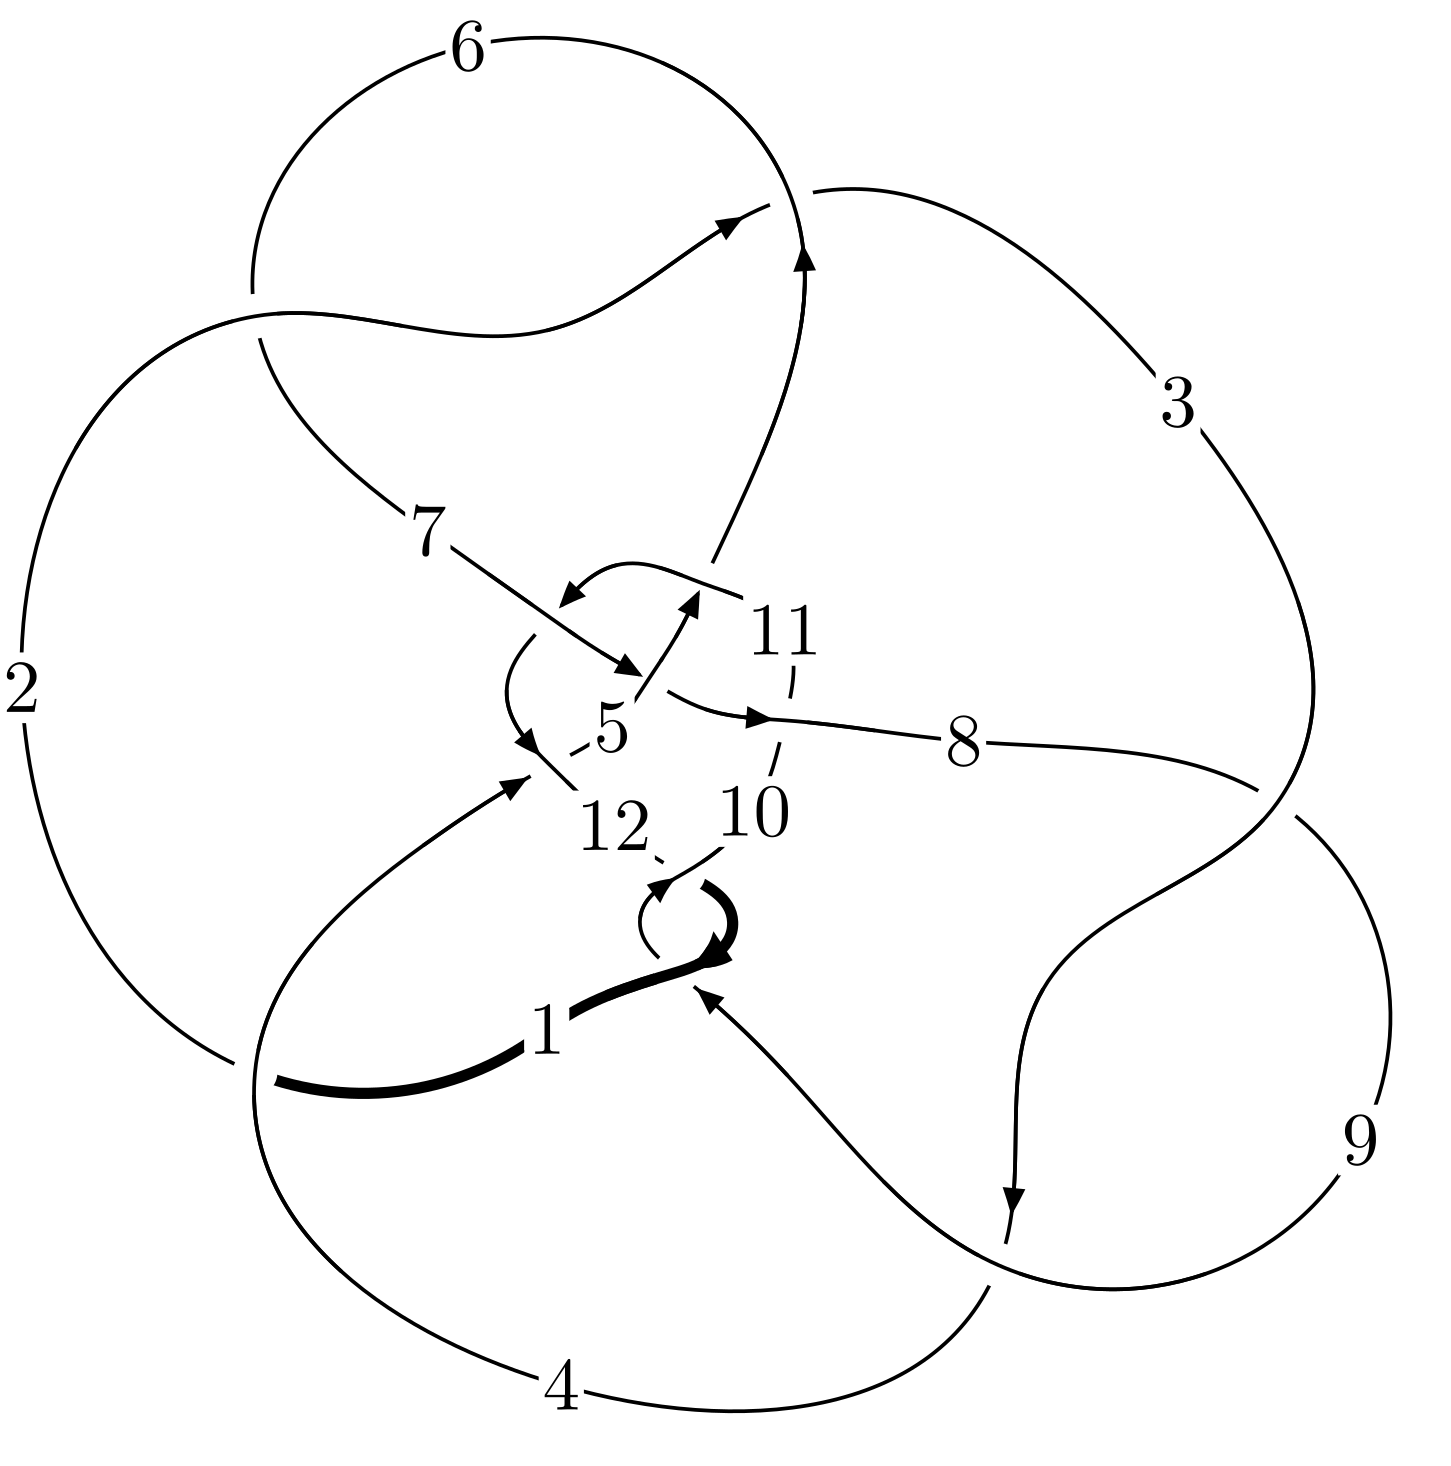
\includegraphics[width=112pt]{../../../GIT/diagram.site/Diagrams/png/1736_12a_0935.png}\\
\ \ \ A knot diagram\footnotemark}&
\allowdisplaybreaks
\textbf{Linearized knot diagam} \\
\cline{2-2}
 &
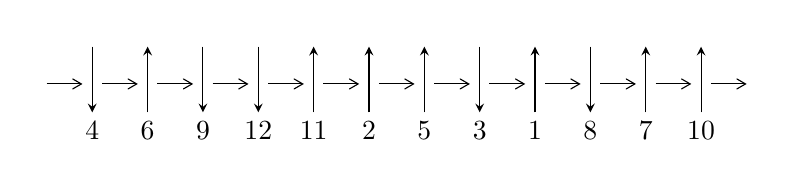
\begin{tikzpicture}[x=20pt, y=17pt]
	% nodes
	\node (C0) at (0, 0) {};
	\node (C1) at (1, 0) {};
	\node (C1U) at (1, +1) {};
	\node (C1D) at (1, -1) {4};

	\node (C2) at (2, 0) {};
	\node (C2U) at (2, +1) {};
	\node (C2D) at (2, -1) {6};

	\node (C3) at (3, 0) {};
	\node (C3U) at (3, +1) {};
	\node (C3D) at (3, -1) {9};

	\node (C4) at (4, 0) {};
	\node (C4U) at (4, +1) {};
	\node (C4D) at (4, -1) {12};

	\node (C5) at (5, 0) {};
	\node (C5U) at (5, +1) {};
	\node (C5D) at (5, -1) {11};

	\node (C6) at (6, 0) {};
	\node (C6U) at (6, +1) {};
	\node (C6D) at (6, -1) {2};

	\node (C7) at (7, 0) {};
	\node (C7U) at (7, +1) {};
	\node (C7D) at (7, -1) {5};

	\node (C8) at (8, 0) {};
	\node (C8U) at (8, +1) {};
	\node (C8D) at (8, -1) {3};

	\node (C9) at (9, 0) {};
	\node (C9U) at (9, +1) {};
	\node (C9D) at (9, -1) {1};

	\node (C10) at (10, 0) {};
	\node (C10U) at (10, +1) {};
	\node (C10D) at (10, -1) {8};

	\node (C11) at (11, 0) {};
	\node (C11U) at (11, +1) {};
	\node (C11D) at (11, -1) {7};

	\node (C12) at (12, 0) {};
	\node (C12U) at (12, +1) {};
	\node (C12D) at (12, -1) {10};
	\node (C13) at (13, 0) {};

	% arrows
	\draw[->,>={angle 60}]
	(C0) edge (C1) (C1) edge (C2) (C2) edge (C3) (C3) edge (C4) (C4) edge (C5) (C5) edge (C6) (C6) edge (C7) (C7) edge (C8) (C8) edge (C9) (C9) edge (C10) (C10) edge (C11) (C11) edge (C12) (C12) edge (C13) ;	\draw[->,>=stealth]
	(C1U) edge (C1D) (C2D) edge (C2U) (C3U) edge (C3D) (C4U) edge (C4D) (C5D) edge (C5U) (C6D) edge (C6U) (C7D) edge (C7U) (C8U) edge (C8D) (C9D) edge (C9U) (C10U) edge (C10D) (C11D) edge (C11U) (C12D) edge (C12U) ;
	\end{tikzpicture} \\
\hhline{~~} \\& 
\textbf{Solving Sequence} \\ \cline{2-2} 
 &
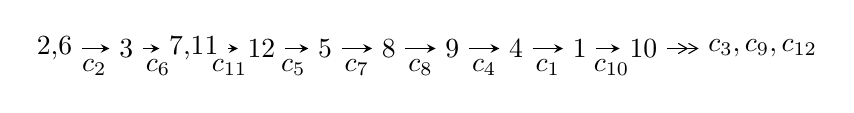
\begin{tikzpicture}[x=23pt, y=7pt]
	% node
	\node (A0) at (-1/8, 0) {2,6};
	\node (A1) at (1, 0) {3};
	\node (A2) at (33/16, 0) {7,11};
	\node (A3) at (25/8, 0) {12};
	\node (A4) at (33/8, 0) {5};
	\node (A5) at (41/8, 0) {8};
	\node (A6) at (49/8, 0) {9};
	\node (A7) at (57/8, 0) {4};
	\node (A8) at (65/8, 0) {1};
	\node (A9) at (73/8, 0) {10};
	\node (C1) at (1/2, -1) {$c_{2}$};
	\node (C2) at (3/2, -1) {$c_{6}$};
	\node (C3) at (21/8, -1) {$c_{11}$};
	\node (C4) at (29/8, -1) {$c_{5}$};
	\node (C5) at (37/8, -1) {$c_{7}$};
	\node (C6) at (45/8, -1) {$c_{8}$};
	\node (C7) at (53/8, -1) {$c_{4}$};
	\node (C8) at (61/8, -1) {$c_{1}$};
	\node (C9) at (69/8, -1) {$c_{10}$};
	\node (A10) at (11, 0) {$c_{3},c_{9},c_{12}$};

	% edge
	\draw[->,>=stealth]	
	(A0) edge (A1) (A1) edge (A2) (A2) edge (A3) (A3) edge (A4) (A4) edge (A5) (A5) edge (A6) (A6) edge (A7) (A7) edge (A8) (A8) edge (A9) ;
	\draw[->>,>={angle 60}]	
	(A9) edge (A10);
\end{tikzpicture} \\ 

\end{tabular} \\

\footnotetext{
The image of knot diagram is generated by the software ``\textbf{Draw programme}" developed by Andrew Bartholomew(\url{http://www.layer8.co.uk/maths/draw/index.htm\#Running-draw}), where we modified some parts for our purpose(\url{https://github.com/CATsTAILs/LinksPainter}).
}\phantom \\ \newline 
\centering \textbf{Ideals for irreducible components\footnotemark of $X_{\text{par}}$} 
 
\begin{align*}
I^u_{1}&=\langle 
7.81900\times10^{985} u^{183}-7.88716\times10^{985} u^{182}+\cdots+6.01907\times10^{985} b+2.13399\times10^{986},\\
\phantom{I^u_{1}}&\phantom{= \langle  }4.35696\times10^{986} u^{183}+3.78145\times10^{985} u^{182}+\cdots+6.01907\times10^{985} a+4.67662\times10^{986},\;u^{184}+u^{183}+\cdots+2 u-1\rangle \\
I^u_{2}&=\langle 
4.73987\times10^{39} u^{49}+1.08770\times10^{39} u^{48}+\cdots+2.55091\times10^{37} b-7.03667\times10^{39},\\
\phantom{I^u_{2}}&\phantom{= \langle  }1.73292\times10^{39} u^{49}+8.72064\times10^{38} u^{48}+\cdots+2.55091\times10^{37} a-5.63180\times10^{39},\;u^{50}+11 u^{48}+\cdots-3 u-1\rangle \\
\\
\end{align*}
\raggedright * 2 irreducible components of $\dim_{\mathbb{C}}=0$, with total 234 representations.\\
\footnotetext{All coefficients of polynomials are rational numbers. But the coefficients are sometimes approximated in decimal forms when there is not enough margin.}
\newpage
\renewcommand{\arraystretch}{1}
\centering \section*{I. $I^u_{1}= \langle 7.82\times10^{985} u^{183}-7.89\times10^{985} u^{182}+\cdots+6.02\times10^{985} b+2.13\times10^{986},\;4.36\times10^{986} u^{183}+3.78\times10^{985} u^{182}+\cdots+6.02\times10^{985} a+4.68\times10^{986},\;u^{184}+u^{183}+\cdots+2 u-1 \rangle$}
\flushleft \textbf{(i) Arc colorings}\\
\begin{tabular}{m{7pt} m{180pt} m{7pt} m{180pt} }
\flushright $a_{2}=$&$\begin{pmatrix}1\\0\end{pmatrix}$ \\
\flushright $a_{6}=$&$\begin{pmatrix}0\\u\end{pmatrix}$ \\
\flushright $a_{3}=$&$\begin{pmatrix}1\\- u^2\end{pmatrix}$ \\
\flushright $a_{7}=$&$\begin{pmatrix}u\\u\end{pmatrix}$ \\
\flushright $a_{11}=$&$\begin{pmatrix}-7.23859 u^{183}-0.628245 u^{182}+\cdots+31.4824 u-7.76968\\-1.29904 u^{183}+1.31036 u^{182}+\cdots+10.0813 u-3.54539\end{pmatrix}$ \\
\flushright $a_{12}=$&$\begin{pmatrix}-10.0540 u^{183}-0.950916 u^{182}+\cdots+45.4239 u-11.7706\\-4.11442 u^{183}+0.987693 u^{182}+\cdots+24.0228 u-7.54633\end{pmatrix}$ \\
\flushright $a_{5}=$&$\begin{pmatrix}0.794746 u^{183}-1.61012 u^{182}+\cdots-35.6727 u+4.52522\\0.0710340 u^{183}-0.574077 u^{182}+\cdots-12.3695 u+0.280865\end{pmatrix}$ \\
\flushright $a_{8}=$&$\begin{pmatrix}9.63510 u^{183}+10.4622 u^{182}+\cdots-24.9001 u-3.41375\\5.88424 u^{183}+5.16103 u^{182}+\cdots-14.7093 u-0.478162\end{pmatrix}$ \\
\flushright $a_{9}=$&$\begin{pmatrix}8.94054 u^{183}+10.3815 u^{182}+\cdots-18.1718 u-3.76267\\5.58760 u^{183}+5.26207 u^{182}+\cdots-12.7870 u-1.09202\end{pmatrix}$ \\
\flushright $a_{4}=$&$\begin{pmatrix}-4.44465 u^{183}-7.51045 u^{182}+\cdots+5.62935 u+5.70928\\-3.45874 u^{183}-3.75085 u^{182}+\cdots+9.20127 u+1.27427\end{pmatrix}$ \\
\flushright $a_{1}=$&$\begin{pmatrix}-21.0857 u^{183}-26.4945 u^{182}+\cdots-0.618143 u+16.9348\\-12.0198 u^{183}-12.1542 u^{182}+\cdots+11.9164 u+3.30388\end{pmatrix}$ \\
\flushright $a_{10}=$&$\begin{pmatrix}24.0006 u^{183}+7.84552 u^{182}+\cdots-102.839 u+29.2947\\6.94557 u^{183}-0.574113 u^{182}+\cdots-38.7545 u+13.4882\end{pmatrix}$\\&\end{tabular}
\flushleft \textbf{(ii) Obstruction class $= -1$}\\~\\
\flushleft \textbf{(iii) Cusp Shapes $= -23.1352 u^{183}-21.1220 u^{182}+\cdots+42.3192 u+9.71975$}\\~\\
\newpage\renewcommand{\arraystretch}{1}
\flushleft \textbf{(iv) u-Polynomials at the component}\newline \\
\begin{tabular}{m{50pt}|m{274pt}}
Crossings & \hspace{64pt}u-Polynomials at each crossing \\
\hline $$\begin{aligned}c_{1}\end{aligned}$$&$\begin{aligned}
&u^{184}-4 u^{183}+\cdots-71040737947 u+8873630559
\end{aligned}$\\
\hline $$\begin{aligned}c_{2},c_{6}\end{aligned}$$&$\begin{aligned}
&u^{184}- u^{183}+\cdots-2 u-1
\end{aligned}$\\
\hline $$\begin{aligned}c_{3},c_{8}\end{aligned}$$&$\begin{aligned}
&u^{184}+u^{183}+\cdots-123190029 u+17977599
\end{aligned}$\\
\hline $$\begin{aligned}c_{4}\end{aligned}$$&$\begin{aligned}
&u^{184}+3 u^{183}+\cdots-822455 u-157289
\end{aligned}$\\
\hline $$\begin{aligned}c_{5}\end{aligned}$$&$\begin{aligned}
&u^{184}+u^{183}+\cdots-22 u-3
\end{aligned}$\\
\hline $$\begin{aligned}c_{7}\end{aligned}$$&$\begin{aligned}
&u^{184}+17 u^{183}+\cdots+108 u+49
\end{aligned}$\\
\hline $$\begin{aligned}c_{9},c_{12}\end{aligned}$$&$\begin{aligned}
&u^{184}-14 u^{183}+\cdots-244560 u+39592
\end{aligned}$\\
\hline $$\begin{aligned}c_{10}\end{aligned}$$&$\begin{aligned}
&u^{184}-13 u^{183}+\cdots+4409 u-1081
\end{aligned}$\\
\hline $$\begin{aligned}c_{11}\end{aligned}$$&$\begin{aligned}
&u^{184}-5 u^{183}+\cdots-57 u-1
\end{aligned}$\\
\hline
\end{tabular}\\~\\
\newpage\renewcommand{\arraystretch}{1}
\flushleft \textbf{(v) Riley Polynomials at the component}\newline \\
\begin{tabular}{m{50pt}|m{274pt}}
Crossings & \hspace{64pt}Riley Polynomials at each crossing \\
\hline $$\begin{aligned}c_{1}\end{aligned}$$&$\begin{aligned}
&y^{184}-48 y^{183}+\cdots-2.97\times10^{21} y+7.87\times10^{19}
\end{aligned}$\\
\hline $$\begin{aligned}c_{2},c_{6}\end{aligned}$$&$\begin{aligned}
&y^{184}+95 y^{183}+\cdots+52 y+1
\end{aligned}$\\
\hline $$\begin{aligned}c_{3},c_{8}\end{aligned}$$&$\begin{aligned}
&y^{184}-145 y^{183}+\cdots-6975999890891991 y+323194065804801
\end{aligned}$\\
\hline $$\begin{aligned}c_{4}\end{aligned}$$&$\begin{aligned}
&y^{184}+57 y^{183}+\cdots+1925713891789 y+24739829521
\end{aligned}$\\
\hline $$\begin{aligned}c_{5}\end{aligned}$$&$\begin{aligned}
&y^{184}-11 y^{183}+\cdots-1072 y+9
\end{aligned}$\\
\hline $$\begin{aligned}c_{7}\end{aligned}$$&$\begin{aligned}
&y^{184}-9 y^{183}+\cdots-210604 y+2401
\end{aligned}$\\
\hline $$\begin{aligned}c_{9},c_{12}\end{aligned}$$&$\begin{aligned}
&y^{184}+120 y^{183}+\cdots+108376113824 y+1567526464
\end{aligned}$\\
\hline $$\begin{aligned}c_{10}\end{aligned}$$&$\begin{aligned}
&y^{184}+19 y^{183}+\cdots+407531937 y+1168561
\end{aligned}$\\
\hline $$\begin{aligned}c_{11}\end{aligned}$$&$\begin{aligned}
&y^{184}-31 y^{183}+\cdots-179 y+1
\end{aligned}$\\
\hline
\end{tabular}\\~\\
\newpage\flushleft \textbf{(vi) Complex Volumes and Cusp Shapes}
$$\begin{array}{c|c|c}  
\text{Solutions to }I^u_{1}& \I (\text{vol} + \sqrt{-1}CS) & \text{Cusp shape}\\
 \hline 
\begin{aligned}
u &= \phantom{-}0.328666 + 0.923922 I \\
a &= -0.337659 - 0.238911 I \\
b &= -0.170979 - 1.240740 I\end{aligned}
 & -4.23227 - 3.34748 I & \phantom{-0.000000 } 0 \\ \hline\begin{aligned}
u &= \phantom{-}0.328666 - 0.923922 I \\
a &= -0.337659 + 0.238911 I \\
b &= -0.170979 + 1.240740 I\end{aligned}
 & -4.23227 + 3.34748 I & \phantom{-0.000000 } 0 \\ \hline\begin{aligned}
u &= \phantom{-}0.281174 + 0.982315 I \\
a &= \phantom{-}0.359990 + 0.210848 I \\
b &= \phantom{-}1.29550 + 1.10202 I\end{aligned}
 & -5.73999 - 1.00560 I & \phantom{-0.000000 } 0 \\ \hline\begin{aligned}
u &= \phantom{-}0.281174 - 0.982315 I \\
a &= \phantom{-}0.359990 - 0.210848 I \\
b &= \phantom{-}1.29550 - 1.10202 I\end{aligned}
 & -5.73999 + 1.00560 I & \phantom{-0.000000 } 0 \\ \hline\begin{aligned}
u &= \phantom{-}0.932460 + 0.245380 I \\
a &= \phantom{-}0.837280 - 1.035300 I \\
b &= \phantom{-}0.0984925 + 0.0643776 I\end{aligned}
 & \phantom{-}1.61224 - 8.91293 I & \phantom{-0.000000 } 0 \\ \hline\begin{aligned}
u &= \phantom{-}0.932460 - 0.245380 I \\
a &= \phantom{-}0.837280 + 1.035300 I \\
b &= \phantom{-}0.0984925 - 0.0643776 I\end{aligned}
 & \phantom{-}1.61224 + 8.91293 I & \phantom{-0.000000 } 0 \\ \hline\begin{aligned}
u &= \phantom{-}0.954235 + 0.402904 I \\
a &= -0.620648 + 1.058490 I \\
b &= -0.0242627 - 0.0856250 I\end{aligned}
 & \phantom{-}4.31278 - 4.19799 I & \phantom{-0.000000 } 0 \\ \hline\begin{aligned}
u &= \phantom{-}0.954235 - 0.402904 I \\
a &= -0.620648 - 1.058490 I \\
b &= -0.0242627 + 0.0856250 I\end{aligned}
 & \phantom{-}4.31278 + 4.19799 I & \phantom{-0.000000 } 0 \\ \hline\begin{aligned}
u &= \phantom{-}1.017440 + 0.228660 I \\
a &= \phantom{-}0.401725 + 0.757657 I \\
b &= \phantom{-}0.317209 + 0.836250 I\end{aligned}
 & \phantom{-}1.02142 + 3.54450 I & \phantom{-0.000000 } 0 \\ \hline\begin{aligned}
u &= \phantom{-}1.017440 - 0.228660 I \\
a &= \phantom{-}0.401725 - 0.757657 I \\
b &= \phantom{-}0.317209 - 0.836250 I\end{aligned}
 & \phantom{-}1.02142 - 3.54450 I & \phantom{-0.000000 } 0\\
 \hline 
 \end{array}$$\newpage$$\begin{array}{c|c|c}  
\text{Solutions to }I^u_{1}& \I (\text{vol} + \sqrt{-1}CS) & \text{Cusp shape}\\
 \hline 
\begin{aligned}
u &= -0.742133 + 0.569313 I \\
a &= \phantom{-}0.882782 + 0.587740 I \\
b &= \phantom{-}0.027380 + 0.526989 I\end{aligned}
 & -0.90654 - 2.78152 I & \phantom{-0.000000 } 0 \\ \hline\begin{aligned}
u &= -0.742133 - 0.569313 I \\
a &= \phantom{-}0.882782 - 0.587740 I \\
b &= \phantom{-}0.027380 - 0.526989 I\end{aligned}
 & -0.90654 + 2.78152 I & \phantom{-0.000000 } 0 \\ \hline\begin{aligned}
u &= -0.395282 + 0.997311 I \\
a &= \phantom{-}0.914452 + 0.863382 I \\
b &= \phantom{-}1.63177 + 0.10048 I\end{aligned}
 & -2.21984 - 0.05198 I & \phantom{-0.000000 } 0 \\ \hline\begin{aligned}
u &= -0.395282 - 0.997311 I \\
a &= \phantom{-}0.914452 - 0.863382 I \\
b &= \phantom{-}1.63177 - 0.10048 I\end{aligned}
 & -2.21984 + 0.05198 I & \phantom{-0.000000 } 0 \\ \hline\begin{aligned}
u &= -0.516582 + 0.945564 I \\
a &= \phantom{-}0.49283 - 1.74278 I \\
b &= \phantom{-}0.82041 - 1.17844 I\end{aligned}
 & \phantom{-}1.36616 - 1.84748 I & \phantom{-0.000000 } 0 \\ \hline\begin{aligned}
u &= -0.516582 - 0.945564 I \\
a &= \phantom{-}0.49283 + 1.74278 I \\
b &= \phantom{-}0.82041 + 1.17844 I\end{aligned}
 & \phantom{-}1.36616 + 1.84748 I & \phantom{-0.000000 } 0 \\ \hline\begin{aligned}
u &= -0.479603 + 0.784159 I \\
a &= -0.897211 - 0.596535 I \\
b &= -0.744257 - 0.439217 I\end{aligned}
 & -1.61001 - 2.03708 I & \phantom{-0.000000 } 0 \\ \hline\begin{aligned}
u &= -0.479603 - 0.784159 I \\
a &= -0.897211 + 0.596535 I \\
b &= -0.744257 + 0.439217 I\end{aligned}
 & -1.61001 + 2.03708 I & \phantom{-0.000000 } 0 \\ \hline\begin{aligned}
u &= -0.407113 + 1.008750 I \\
a &= -0.98531 + 1.47233 I \\
b &= -1.52746 + 1.13774 I\end{aligned}
 & -2.18677 - 5.95841 I & \phantom{-0.000000 } 0 \\ \hline\begin{aligned}
u &= -0.407113 - 1.008750 I \\
a &= -0.98531 - 1.47233 I \\
b &= -1.52746 - 1.13774 I\end{aligned}
 & -2.18677 + 5.95841 I & \phantom{-0.000000 } 0\\
 \hline 
 \end{array}$$\newpage$$\begin{array}{c|c|c}  
\text{Solutions to }I^u_{1}& \I (\text{vol} + \sqrt{-1}CS) & \text{Cusp shape}\\
 \hline 
\begin{aligned}
u &= \phantom{-}0.386401 + 0.817211 I \\
a &= -0.203956 + 0.830260 I \\
b &= -0.159541 - 1.196870 I\end{aligned}
 & \phantom{-}2.45806 + 0.61893 I & \phantom{-0.000000 } 0 \\ \hline\begin{aligned}
u &= \phantom{-}0.386401 - 0.817211 I \\
a &= -0.203956 - 0.830260 I \\
b &= -0.159541 + 1.196870 I\end{aligned}
 & \phantom{-}2.45806 - 0.61893 I & \phantom{-0.000000 } 0 \\ \hline\begin{aligned}
u &= -1.046150 + 0.332738 I \\
a &= -0.1227220 + 0.0159749 I \\
b &= \phantom{-}0.424953 - 0.507347 I\end{aligned}
 & \phantom{-}0.29483 - 2.54882 I & \phantom{-0.000000 } 0 \\ \hline\begin{aligned}
u &= -1.046150 - 0.332738 I \\
a &= -0.1227220 - 0.0159749 I \\
b &= \phantom{-}0.424953 + 0.507347 I\end{aligned}
 & \phantom{-}0.29483 + 2.54882 I & \phantom{-0.000000 } 0 \\ \hline\begin{aligned}
u &= \phantom{-}0.305621 + 0.839689 I \\
a &= \phantom{-}0.451118 - 0.745475 I \\
b &= \phantom{-}0.53162 + 1.38599 I\end{aligned}
 & -0.04717 + 5.21582 I & \phantom{-0.000000 } 0 \\ \hline\begin{aligned}
u &= \phantom{-}0.305621 - 0.839689 I \\
a &= \phantom{-}0.451118 + 0.745475 I \\
b &= \phantom{-}0.53162 - 1.38599 I\end{aligned}
 & -0.04717 - 5.21582 I & \phantom{-0.000000 } 0 \\ \hline\begin{aligned}
u &= \phantom{-}0.102778 + 1.102560 I \\
a &= -0.289562 - 0.337758 I \\
b &= -0.915694 - 0.515381 I\end{aligned}
 & -1.38744 - 1.57426 I & \phantom{-0.000000 } 0 \\ \hline\begin{aligned}
u &= \phantom{-}0.102778 - 1.102560 I \\
a &= -0.289562 + 0.337758 I \\
b &= -0.915694 + 0.515381 I\end{aligned}
 & -1.38744 + 1.57426 I & \phantom{-0.000000 } 0 \\ \hline\begin{aligned}
u &= -0.836195 + 0.738359 I \\
a &= -0.022615 - 0.420518 I \\
b &= \phantom{-}0.530676 - 0.335424 I\end{aligned}
 & \phantom{-}0.53731 - 2.71696 I & \phantom{-0.000000 } 0 \\ \hline\begin{aligned}
u &= -0.836195 - 0.738359 I \\
a &= -0.022615 + 0.420518 I \\
b &= \phantom{-}0.530676 + 0.335424 I\end{aligned}
 & \phantom{-}0.53731 + 2.71696 I & \phantom{-0.000000 } 0\\
 \hline 
 \end{array}$$\newpage$$\begin{array}{c|c|c}  
\text{Solutions to }I^u_{1}& \I (\text{vol} + \sqrt{-1}CS) & \text{Cusp shape}\\
 \hline 
\begin{aligned}
u &= -1.058620 + 0.359379 I \\
a &= -0.629799 + 0.183331 I \\
b &= \phantom{-}0.0755610 + 0.0941588 I\end{aligned}
 & \phantom{-}2.95384 - 4.28359 I & \phantom{-0.000000 } 0 \\ \hline\begin{aligned}
u &= -1.058620 - 0.359379 I \\
a &= -0.629799 - 0.183331 I \\
b &= \phantom{-}0.0755610 - 0.0941588 I\end{aligned}
 & \phantom{-}2.95384 + 4.28359 I & \phantom{-0.000000 } 0 \\ \hline\begin{aligned}
u &= -0.234597 + 1.093200 I \\
a &= \phantom{-}0.855601 + 0.763460 I \\
b &= \phantom{-}2.06976 + 0.90235 I\end{aligned}
 & -5.95286 - 2.79198 I & \phantom{-0.000000 } 0 \\ \hline\begin{aligned}
u &= -0.234597 - 1.093200 I \\
a &= \phantom{-}0.855601 - 0.763460 I \\
b &= \phantom{-}2.06976 - 0.90235 I\end{aligned}
 & -5.95286 + 2.79198 I & \phantom{-0.000000 } 0 \\ \hline\begin{aligned}
u &= -0.875789 + 0.085333 I \\
a &= \phantom{-}0.980339 - 0.393564 I \\
b &= -0.003387 - 0.152822 I\end{aligned}
 & \phantom{-}2.58017 - 0.01612 I & \phantom{-0.000000 } 0 \\ \hline\begin{aligned}
u &= -0.875789 - 0.085333 I \\
a &= \phantom{-}0.980339 + 0.393564 I \\
b &= -0.003387 + 0.152822 I\end{aligned}
 & \phantom{-}2.58017 + 0.01612 I & \phantom{-0.000000 } 0 \\ \hline\begin{aligned}
u &= -0.716125 + 0.500928 I \\
a &= -0.751351 - 0.879330 I \\
b &= \phantom{-}0.160617 - 0.584912 I\end{aligned}
 & \phantom{-}0.14160 - 2.74021 I & \phantom{-0.000000 } 0 \\ \hline\begin{aligned}
u &= -0.716125 - 0.500928 I \\
a &= -0.751351 + 0.879330 I \\
b &= \phantom{-}0.160617 + 0.584912 I\end{aligned}
 & \phantom{-}0.14160 + 2.74021 I & \phantom{-0.000000 } 0 \\ \hline\begin{aligned}
u &= -0.076671 + 0.866866 I \\
a &= -0.24748 - 1.49759 I \\
b &= -1.209750 - 0.282047 I\end{aligned}
 & -4.71081 + 1.61436 I & \phantom{-0.000000 } 0 \\ \hline\begin{aligned}
u &= -0.076671 - 0.866866 I \\
a &= -0.24748 + 1.49759 I \\
b &= -1.209750 + 0.282047 I\end{aligned}
 & -4.71081 - 1.61436 I & \phantom{-0.000000 } 0\\
 \hline 
 \end{array}$$\newpage$$\begin{array}{c|c|c}  
\text{Solutions to }I^u_{1}& \I (\text{vol} + \sqrt{-1}CS) & \text{Cusp shape}\\
 \hline 
\begin{aligned}
u &= -0.439982 + 1.046660 I \\
a &= -1.268990 - 0.479427 I \\
b &= -1.88839 - 0.77911 I\end{aligned}
 & -0.87427 - 3.56380 I & \phantom{-0.000000 } 0 \\ \hline\begin{aligned}
u &= -0.439982 - 1.046660 I \\
a &= -1.268990 + 0.479427 I \\
b &= -1.88839 + 0.77911 I\end{aligned}
 & -0.87427 + 3.56380 I & \phantom{-0.000000 } 0 \\ \hline\begin{aligned}
u &= -0.559459 + 0.990612 I \\
a &= \phantom{-}1.076900 + 0.316696 I \\
b &= \phantom{-}1.35625 + 0.67086 I\end{aligned}
 & -1.22853 - 2.11504 I & \phantom{-0.000000 } 0 \\ \hline\begin{aligned}
u &= -0.559459 - 0.990612 I \\
a &= \phantom{-}1.076900 - 0.316696 I \\
b &= \phantom{-}1.35625 - 0.67086 I\end{aligned}
 & -1.22853 + 2.11504 I & \phantom{-0.000000 } 0 \\ \hline\begin{aligned}
u &= \phantom{-}0.048454 + 0.848204 I \\
a &= -0.779682 - 1.070800 I \\
b &= -1.145820 + 0.165807 I\end{aligned}
 & -1.66325 - 2.67840 I & \phantom{-0.000000 } 0 \\ \hline\begin{aligned}
u &= \phantom{-}0.048454 - 0.848204 I \\
a &= -0.779682 + 1.070800 I \\
b &= -1.145820 - 0.165807 I\end{aligned}
 & -1.66325 + 2.67840 I & \phantom{-0.000000 } 0 \\ \hline\begin{aligned}
u &= \phantom{-}0.684155 + 0.497669 I \\
a &= \phantom{-}0.404608 + 0.408649 I \\
b &= -0.174427 + 0.086705 I\end{aligned}
 & -1.73029 - 0.93389 I & \phantom{-0.000000 } 0 \\ \hline\begin{aligned}
u &= \phantom{-}0.684155 - 0.497669 I \\
a &= \phantom{-}0.404608 - 0.408649 I \\
b &= -0.174427 - 0.086705 I\end{aligned}
 & -1.73029 + 0.93389 I & \phantom{-0.000000 } 0 \\ \hline\begin{aligned}
u &= \phantom{-}0.098377 + 0.839720 I \\
a &= -0.405353 + 1.132110 I \\
b &= \phantom{-}0.260415 - 1.036450 I\end{aligned}
 & -3.45130 + 5.18108 I & \phantom{-0.000000 } 0 \\ \hline\begin{aligned}
u &= \phantom{-}0.098377 - 0.839720 I \\
a &= -0.405353 - 1.132110 I \\
b &= \phantom{-}0.260415 + 1.036450 I\end{aligned}
 & -3.45130 - 5.18108 I & \phantom{-0.000000 } 0\\
 \hline 
 \end{array}$$\newpage$$\begin{array}{c|c|c}  
\text{Solutions to }I^u_{1}& \I (\text{vol} + \sqrt{-1}CS) & \text{Cusp shape}\\
 \hline 
\begin{aligned}
u &= -0.234639 + 1.136980 I \\
a &= -0.392035 - 0.377420 I \\
b &= -0.875694 - 0.346315 I\end{aligned}
 & -1.33306 - 1.70403 I & \phantom{-0.000000 } 0 \\ \hline\begin{aligned}
u &= -0.234639 - 1.136980 I \\
a &= -0.392035 + 0.377420 I \\
b &= -0.875694 + 0.346315 I\end{aligned}
 & -1.33306 + 1.70403 I & \phantom{-0.000000 } 0 \\ \hline\begin{aligned}
u &= -0.367582 + 1.122900 I \\
a &= -1.116720 - 0.536632 I \\
b &= -1.94737 - 0.92939 I\end{aligned}
 & -1.12999 - 3.80246 I & \phantom{-0.000000 } 0 \\ \hline\begin{aligned}
u &= -0.367582 - 1.122900 I \\
a &= -1.116720 + 0.536632 I \\
b &= -1.94737 + 0.92939 I\end{aligned}
 & -1.12999 + 3.80246 I & \phantom{-0.000000 } 0 \\ \hline\begin{aligned}
u &= \phantom{-}0.605279 + 1.015050 I \\
a &= -0.999021 + 0.169632 I \\
b &= -2.33491 + 0.60399 I\end{aligned}
 & -3.63955 + 7.18297 I & \phantom{-0.000000 } 0 \\ \hline\begin{aligned}
u &= \phantom{-}0.605279 - 1.015050 I \\
a &= -0.999021 - 0.169632 I \\
b &= -2.33491 - 0.60399 I\end{aligned}
 & -3.63955 - 7.18297 I & \phantom{-0.000000 } 0 \\ \hline\begin{aligned}
u &= \phantom{-}0.260915 + 0.765957 I \\
a &= -0.036896 + 0.185567 I \\
b &= -2.10271 + 0.45733 I\end{aligned}
 & \phantom{-}0.21605 - 2.34849 I & \phantom{-0.000000 } 0 \\ \hline\begin{aligned}
u &= \phantom{-}0.260915 - 0.765957 I \\
a &= -0.036896 - 0.185567 I \\
b &= -2.10271 - 0.45733 I\end{aligned}
 & \phantom{-}0.21605 + 2.34849 I & \phantom{-0.000000 } 0 \\ \hline\begin{aligned}
u &= \phantom{-}0.537647 + 1.072600 I \\
a &= \phantom{-}1.317540 - 0.141462 I \\
b &= \phantom{-}2.34754 - 0.83714 I\end{aligned}
 & -2.86655 + 9.64651 I & \phantom{-0.000000 } 0 \\ \hline\begin{aligned}
u &= \phantom{-}0.537647 - 1.072600 I \\
a &= \phantom{-}1.317540 + 0.141462 I \\
b &= \phantom{-}2.34754 + 0.83714 I\end{aligned}
 & -2.86655 - 9.64651 I & \phantom{-0.000000 } 0\\
 \hline 
 \end{array}$$\newpage$$\begin{array}{c|c|c}  
\text{Solutions to }I^u_{1}& \I (\text{vol} + \sqrt{-1}CS) & \text{Cusp shape}\\
 \hline 
\begin{aligned}
u &= \phantom{-}0.333919 + 0.717506 I \\
a &= \phantom{-}0.268066 - 0.342195 I \\
b &= \phantom{-}2.59020 - 0.47265 I\end{aligned}
 & \phantom{-}2.78920 + 2.76787 I & \phantom{-0.000000 } 0 \\ \hline\begin{aligned}
u &= \phantom{-}0.333919 - 0.717506 I \\
a &= \phantom{-}0.268066 + 0.342195 I \\
b &= \phantom{-}2.59020 + 0.47265 I\end{aligned}
 & \phantom{-}2.78920 - 2.76787 I & \phantom{-0.000000 } 0 \\ \hline\begin{aligned}
u &= -0.333894 + 1.167410 I \\
a &= \phantom{-}1.129530 + 0.411509 I \\
b &= \phantom{-}2.00594 + 1.02466 I\end{aligned}
 & -2.07419 - 7.73209 I & \phantom{-0.000000 } 0 \\ \hline\begin{aligned}
u &= -0.333894 - 1.167410 I \\
a &= \phantom{-}1.129530 - 0.411509 I \\
b &= \phantom{-}2.00594 - 1.02466 I\end{aligned}
 & -2.07419 + 7.73209 I & \phantom{-0.000000 } 0 \\ \hline\begin{aligned}
u &= \phantom{-}0.501635 + 1.108730 I \\
a &= -1.353990 + 0.309421 I \\
b &= -2.23528 + 0.81907 I\end{aligned}
 & -1.99883 + 8.46741 I & \phantom{-0.000000 } 0 \\ \hline\begin{aligned}
u &= \phantom{-}0.501635 - 1.108730 I \\
a &= -1.353990 - 0.309421 I \\
b &= -2.23528 - 0.81907 I\end{aligned}
 & -1.99883 - 8.46741 I & \phantom{-0.000000 } 0 \\ \hline\begin{aligned}
u &= -0.419293 + 1.144830 I \\
a &= -0.812068 + 0.252464 I \\
b &= -2.07568 - 0.85191 I\end{aligned}
 & -8.69619 - 9.59606 I & \phantom{-0.000000 } 0 \\ \hline\begin{aligned}
u &= -0.419293 - 1.144830 I \\
a &= -0.812068 - 0.252464 I \\
b &= -2.07568 + 0.85191 I\end{aligned}
 & -8.69619 + 9.59606 I & \phantom{-0.000000 } 0 \\ \hline\begin{aligned}
u &= \phantom{-}0.640452 + 0.434618 I \\
a &= -0.46007 + 1.69091 I \\
b &= \phantom{-}0.486726 + 0.141249 I\end{aligned}
 & -0.97778 - 5.02063 I & \phantom{-0.000000 } 0 \\ \hline\begin{aligned}
u &= \phantom{-}0.640452 - 0.434618 I \\
a &= -0.46007 - 1.69091 I \\
b &= \phantom{-}0.486726 - 0.141249 I\end{aligned}
 & -0.97778 + 5.02063 I & \phantom{-0.000000 } 0\\
 \hline 
 \end{array}$$\newpage$$\begin{array}{c|c|c}  
\text{Solutions to }I^u_{1}& \I (\text{vol} + \sqrt{-1}CS) & \text{Cusp shape}\\
 \hline 
\begin{aligned}
u &= -0.028026 + 0.762209 I \\
a &= -0.34995 + 2.09230 I \\
b &= \phantom{-}0.049671 + 0.551414 I\end{aligned}
 & \phantom{-}1.20764 + 2.00995 I & \phantom{-0.000000 } 0 \\ \hline\begin{aligned}
u &= -0.028026 - 0.762209 I \\
a &= -0.34995 - 2.09230 I \\
b &= \phantom{-}0.049671 - 0.551414 I\end{aligned}
 & \phantom{-}1.20764 - 2.00995 I & \phantom{-0.000000 } 0 \\ \hline\begin{aligned}
u &= \phantom{-}0.435567 + 1.158280 I \\
a &= -0.49408 - 1.76943 I \\
b &= -0.89729 - 1.21336 I\end{aligned}
 & -5.86458 + 11.37010 I & \phantom{-0.000000 } 0 \\ \hline\begin{aligned}
u &= \phantom{-}0.435567 - 1.158280 I \\
a &= -0.49408 + 1.76943 I \\
b &= -0.89729 + 1.21336 I\end{aligned}
 & -5.86458 - 11.37010 I & \phantom{-0.000000 } 0 \\ \hline\begin{aligned}
u &= -1.014410 + 0.720047 I \\
a &= \phantom{-}0.239715 + 1.213540 I \\
b &= \phantom{-}0.0238577 + 0.1296900 I\end{aligned}
 & -5.33470 + 0.59771 I & \phantom{-0.000000 } 0 \\ \hline\begin{aligned}
u &= -1.014410 - 0.720047 I \\
a &= \phantom{-}0.239715 - 1.213540 I \\
b &= \phantom{-}0.0238577 - 0.1296900 I\end{aligned}
 & -5.33470 - 0.59771 I & \phantom{-0.000000 } 0 \\ \hline\begin{aligned}
u &= -0.410857 + 1.178470 I \\
a &= \phantom{-}0.375001 + 0.455285 I \\
b &= \phantom{-}1.18080 - 1.41938 I\end{aligned}
 & -6.47721 - 10.97930 I & \phantom{-0.000000 } 0 \\ \hline\begin{aligned}
u &= -0.410857 - 1.178470 I \\
a &= \phantom{-}0.375001 - 0.455285 I \\
b &= \phantom{-}1.18080 + 1.41938 I\end{aligned}
 & -6.47721 + 10.97930 I & \phantom{-0.000000 } 0 \\ \hline\begin{aligned}
u &= -0.644231 + 0.372872 I \\
a &= \phantom{-}0.447550 - 0.173413 I \\
b &= -1.267090 + 0.225983 I\end{aligned}
 & -5.33586 - 6.28246 I & \phantom{-0.000000 } 0 \\ \hline\begin{aligned}
u &= -0.644231 - 0.372872 I \\
a &= \phantom{-}0.447550 + 0.173413 I \\
b &= -1.267090 - 0.225983 I\end{aligned}
 & -5.33586 + 6.28246 I & \phantom{-0.000000 } 0\\
 \hline 
 \end{array}$$\newpage$$\begin{array}{c|c|c}  
\text{Solutions to }I^u_{1}& \I (\text{vol} + \sqrt{-1}CS) & \text{Cusp shape}\\
 \hline 
\begin{aligned}
u &= \phantom{-}0.438705 + 1.177180 I \\
a &= -1.54908 + 0.43391 I \\
b &= -2.10095 + 0.63619 I\end{aligned}
 & -2.94278 + 7.44361 I & \phantom{-0.000000 } 0 \\ \hline\begin{aligned}
u &= \phantom{-}0.438705 - 1.177180 I \\
a &= -1.54908 - 0.43391 I \\
b &= -2.10095 - 0.63619 I\end{aligned}
 & -2.94278 - 7.44361 I & \phantom{-0.000000 } 0 \\ \hline\begin{aligned}
u &= -0.382326 + 1.197740 I \\
a &= \phantom{-}0.721448 + 0.109899 I \\
b &= \phantom{-}2.03743 + 0.82252 I\end{aligned}
 & -4.22919 - 6.26560 I & \phantom{-0.000000 } 0 \\ \hline\begin{aligned}
u &= -0.382326 - 1.197740 I \\
a &= \phantom{-}0.721448 - 0.109899 I \\
b &= \phantom{-}2.03743 - 0.82252 I\end{aligned}
 & -4.22919 + 6.26560 I & \phantom{-0.000000 } 0 \\ \hline\begin{aligned}
u &= -0.033716 + 0.738210 I \\
a &= \phantom{-}0.84910 - 1.98834 I \\
b &= \phantom{-}0.574428 - 0.270139 I\end{aligned}
 & \phantom{-}0.24310 + 6.09666 I & \phantom{-0.000000 } 0 \\ \hline\begin{aligned}
u &= -0.033716 - 0.738210 I \\
a &= \phantom{-}0.84910 + 1.98834 I \\
b &= \phantom{-}0.574428 + 0.270139 I\end{aligned}
 & \phantom{-}0.24310 - 6.09666 I & \phantom{-0.000000 } 0 \\ \hline\begin{aligned}
u &= \phantom{-}0.529876 + 1.145710 I \\
a &= -0.708720 - 0.047149 I \\
b &= -1.72054 - 0.23689 I\end{aligned}
 & -7.39934 + 3.53210 I & \phantom{-0.000000 } 0 \\ \hline\begin{aligned}
u &= \phantom{-}0.529876 - 1.145710 I \\
a &= -0.708720 + 0.047149 I \\
b &= -1.72054 + 0.23689 I\end{aligned}
 & -7.39934 - 3.53210 I & \phantom{-0.000000 } 0 \\ \hline\begin{aligned}
u &= \phantom{-}0.442939 + 1.182310 I \\
a &= \phantom{-}0.866422 + 0.102242 I \\
b &= \phantom{-}2.17875 - 0.05556 I\end{aligned}
 & -7.80553 + 4.86185 I & \phantom{-0.000000 } 0 \\ \hline\begin{aligned}
u &= \phantom{-}0.442939 - 1.182310 I \\
a &= \phantom{-}0.866422 - 0.102242 I \\
b &= \phantom{-}2.17875 + 0.05556 I\end{aligned}
 & -7.80553 - 4.86185 I & \phantom{-0.000000 } 0\\
 \hline 
 \end{array}$$\newpage$$\begin{array}{c|c|c}  
\text{Solutions to }I^u_{1}& \I (\text{vol} + \sqrt{-1}CS) & \text{Cusp shape}\\
 \hline 
\begin{aligned}
u &= \phantom{-}0.393652 + 1.211750 I \\
a &= \phantom{-}0.21775 + 1.75107 I \\
b &= \phantom{-}0.443968 + 1.025100 I\end{aligned}
 & -0.87631 + 4.82402 I & \phantom{-0.000000 } 0 \\ \hline\begin{aligned}
u &= \phantom{-}0.393652 - 1.211750 I \\
a &= \phantom{-}0.21775 - 1.75107 I \\
b &= \phantom{-}0.443968 - 1.025100 I\end{aligned}
 & -0.87631 - 4.82402 I & \phantom{-0.000000 } 0 \\ \hline\begin{aligned}
u &= -0.087241 + 0.719984 I \\
a &= -2.34275 + 0.61256 I \\
b &= -2.33447 + 0.79117 I\end{aligned}
 & -0.53378 + 3.17236 I & \phantom{-0.000000 } 0 \\ \hline\begin{aligned}
u &= -0.087241 - 0.719984 I \\
a &= -2.34275 - 0.61256 I \\
b &= -2.33447 - 0.79117 I\end{aligned}
 & -0.53378 - 3.17236 I & \phantom{-0.000000 } 0 \\ \hline\begin{aligned}
u &= -0.748779 + 1.038760 I \\
a &= \phantom{-}0.365359 - 0.150185 I \\
b &= \phantom{-}0.770047 - 0.017026 I\end{aligned}
 & \phantom{-}0.40911 - 2.74174 I & \phantom{-0.000000 } 0 \\ \hline\begin{aligned}
u &= -0.748779 - 1.038760 I \\
a &= \phantom{-}0.365359 + 0.150185 I \\
b &= \phantom{-}0.770047 + 0.017026 I\end{aligned}
 & \phantom{-}0.40911 + 2.74174 I & \phantom{-0.000000 } 0 \\ \hline\begin{aligned}
u &= -1.229120 + 0.362344 I \\
a &= \phantom{-}0.465705 + 0.983824 I \\
b &= -0.0368071 - 0.0127765 I\end{aligned}
 & -3.4044 + 14.3626 I & \phantom{-0.000000 } 0 \\ \hline\begin{aligned}
u &= -1.229120 - 0.362344 I \\
a &= \phantom{-}0.465705 - 0.983824 I \\
b &= -0.0368071 + 0.0127765 I\end{aligned}
 & -3.4044 - 14.3626 I & \phantom{-0.000000 } 0 \\ \hline\begin{aligned}
u &= \phantom{-}0.466760 + 1.194170 I \\
a &= \phantom{-}1.33115 - 0.73487 I \\
b &= \phantom{-}2.18556 - 0.70231 I\end{aligned}
 & -9.5040 + 10.9406 I & \phantom{-0.000000 } 0 \\ \hline\begin{aligned}
u &= \phantom{-}0.466760 - 1.194170 I \\
a &= \phantom{-}1.33115 + 0.73487 I \\
b &= \phantom{-}2.18556 + 0.70231 I\end{aligned}
 & -9.5040 - 10.9406 I & \phantom{-0.000000 } 0\\
 \hline 
 \end{array}$$\newpage$$\begin{array}{c|c|c}  
\text{Solutions to }I^u_{1}& \I (\text{vol} + \sqrt{-1}CS) & \text{Cusp shape}\\
 \hline 
\begin{aligned}
u &= \phantom{-}0.558332 + 1.161560 I \\
a &= \phantom{-}0.443192 + 0.167744 I \\
b &= \phantom{-}0.501884 + 0.269382 I\end{aligned}
 & -2.20499 - 1.02816 I & \phantom{-0.000000 } 0 \\ \hline\begin{aligned}
u &= \phantom{-}0.558332 - 1.161560 I \\
a &= \phantom{-}0.443192 - 0.167744 I \\
b &= \phantom{-}0.501884 - 0.269382 I\end{aligned}
 & -2.20499 + 1.02816 I & \phantom{-0.000000 } 0 \\ \hline\begin{aligned}
u &= -0.285330 + 1.258170 I \\
a &= -0.637101 - 0.450925 I \\
b &= -1.89429 - 1.05798 I\end{aligned}
 & -6.47059 - 5.52853 I & \phantom{-0.000000 } 0 \\ \hline\begin{aligned}
u &= -0.285330 - 1.258170 I \\
a &= -0.637101 + 0.450925 I \\
b &= -1.89429 + 1.05798 I\end{aligned}
 & -6.47059 + 5.52853 I & \phantom{-0.000000 } 0 \\ \hline\begin{aligned}
u &= \phantom{-}0.149208 + 0.690518 I \\
a &= \phantom{-}0.91398 - 1.08084 I \\
b &= \phantom{-}0.507391 + 0.855322 I\end{aligned}
 & -0.72543 + 4.34633 I & \phantom{-0.000000 } 0 \\ \hline\begin{aligned}
u &= \phantom{-}0.149208 - 0.690518 I \\
a &= \phantom{-}0.91398 + 1.08084 I \\
b &= \phantom{-}0.507391 - 0.855322 I\end{aligned}
 & -0.72543 - 4.34633 I & \phantom{-0.000000 } 0 \\ \hline\begin{aligned}
u &= -0.387714 + 1.234250 I \\
a &= -0.270639 - 0.660009 I \\
b &= -0.655789 + 1.049870 I\end{aligned}
 & -1.42165 - 5.04521 I & \phantom{-0.000000 } 0 \\ \hline\begin{aligned}
u &= -0.387714 - 1.234250 I \\
a &= -0.270639 + 0.660009 I \\
b &= -0.655789 - 1.049870 I\end{aligned}
 & -1.42165 + 5.04521 I & \phantom{-0.000000 } 0 \\ \hline\begin{aligned}
u &= -0.531578 + 1.185050 I \\
a &= \phantom{-}0.372724 + 0.181043 I \\
b &= \phantom{-}1.17027 - 0.84612 I\end{aligned}
 & -7.86948 + 1.40734 I & \phantom{-0.000000 } 0 \\ \hline\begin{aligned}
u &= -0.531578 - 1.185050 I \\
a &= \phantom{-}0.372724 - 0.181043 I \\
b &= \phantom{-}1.17027 + 0.84612 I\end{aligned}
 & -7.86948 - 1.40734 I & \phantom{-0.000000 } 0\\
 \hline 
 \end{array}$$\newpage$$\begin{array}{c|c|c}  
\text{Solutions to }I^u_{1}& \I (\text{vol} + \sqrt{-1}CS) & \text{Cusp shape}\\
 \hline 
\begin{aligned}
u &= \phantom{-}0.431204 + 1.225640 I \\
a &= \phantom{-}1.319220 + 0.005708 I \\
b &= \phantom{-}1.65394 - 0.15921 I\end{aligned}
 & -2.77505 + 1.47441 I & \phantom{-0.000000 } 0 \\ \hline\begin{aligned}
u &= \phantom{-}0.431204 - 1.225640 I \\
a &= \phantom{-}1.319220 - 0.005708 I \\
b &= \phantom{-}1.65394 + 0.15921 I\end{aligned}
 & -2.77505 - 1.47441 I & \phantom{-0.000000 } 0 \\ \hline\begin{aligned}
u &= -0.626526 + 0.312049 I \\
a &= -1.17416 + 0.87841 I \\
b &= -2.10004 - 0.32376 I\end{aligned}
 & -2.84820 - 7.42093 I & \phantom{-0.000000 } 0 \\ \hline\begin{aligned}
u &= -0.626526 - 0.312049 I \\
a &= -1.17416 - 0.87841 I \\
b &= -2.10004 + 0.32376 I\end{aligned}
 & -2.84820 + 7.42093 I & \phantom{-0.000000 } 0 \\ \hline\begin{aligned}
u &= \phantom{-}0.680546 + 0.036182 I \\
a &= -1.43002 - 1.24968 I \\
b &= -0.722558 - 0.480001 I\end{aligned}
 & -6.14873 + 6.63023 I & \phantom{-0.000000 } 0 \\ \hline\begin{aligned}
u &= \phantom{-}0.680546 - 0.036182 I \\
a &= -1.43002 + 1.24968 I \\
b &= -0.722558 + 0.480001 I\end{aligned}
 & -6.14873 - 6.63023 I & \phantom{-0.000000 } 0 \\ \hline\begin{aligned}
u &= \phantom{-}0.678918 + 0.002816 I \\
a &= -0.217258 + 1.174120 I \\
b &= \phantom{-}0.149928 - 0.325133 I\end{aligned}
 & -4.46591 - 0.70645 I & \phantom{-0.000000 } 0 \\ \hline\begin{aligned}
u &= \phantom{-}0.678918 - 0.002816 I \\
a &= -0.217258 - 1.174120 I \\
b &= \phantom{-}0.149928 + 0.325133 I\end{aligned}
 & -4.46591 + 0.70645 I & \phantom{-0.000000 } 0 \\ \hline\begin{aligned}
u &= \phantom{-}0.504277 + 0.453511 I \\
a &= \phantom{-}0.16964 - 1.44820 I \\
b &= -0.346566 + 0.366879 I\end{aligned}
 & -2.28472 - 2.65617 I & \phantom{-0.000000 } 0 \\ \hline\begin{aligned}
u &= \phantom{-}0.504277 - 0.453511 I \\
a &= \phantom{-}0.16964 + 1.44820 I \\
b &= -0.346566 - 0.366879 I\end{aligned}
 & -2.28472 + 2.65617 I & \phantom{-0.000000 } 0\\
 \hline 
 \end{array}$$\newpage$$\begin{array}{c|c|c}  
\text{Solutions to }I^u_{1}& \I (\text{vol} + \sqrt{-1}CS) & \text{Cusp shape}\\
 \hline 
\begin{aligned}
u &= \phantom{-}0.475985 + 1.235950 I \\
a &= -0.856491 - 0.678835 I \\
b &= -1.260310 - 0.622777 I\end{aligned}
 & -9.45377 - 2.03390 I & \phantom{-0.000000 } 0 \\ \hline\begin{aligned}
u &= \phantom{-}0.475985 - 1.235950 I \\
a &= -0.856491 + 0.678835 I \\
b &= -1.260310 + 0.622777 I\end{aligned}
 & -9.45377 + 2.03390 I & \phantom{-0.000000 } 0 \\ \hline\begin{aligned}
u &= \phantom{-}0.621220 + 1.187460 I \\
a &= \phantom{-}1.041710 - 0.347191 I \\
b &= \phantom{-}2.18949 - 0.71861 I\end{aligned}
 & \phantom{-}1.81905 + 9.95689 I & \phantom{-0.000000 } 0 \\ \hline\begin{aligned}
u &= \phantom{-}0.621220 - 1.187460 I \\
a &= \phantom{-}1.041710 + 0.347191 I \\
b &= \phantom{-}2.18949 + 0.71861 I\end{aligned}
 & \phantom{-}1.81905 - 9.95689 I & \phantom{-0.000000 } 0 \\ \hline\begin{aligned}
u &= -0.486092 + 1.258670 I \\
a &= -0.384993 - 0.183344 I \\
b &= -1.46208 + 0.06014 I\end{aligned}
 & -3.25832 - 3.00238 I & \phantom{-0.000000 } 0 \\ \hline\begin{aligned}
u &= -0.486092 - 1.258670 I \\
a &= -0.384993 + 0.183344 I \\
b &= -1.46208 - 0.06014 I\end{aligned}
 & -3.25832 + 3.00238 I & \phantom{-0.000000 } 0 \\ \hline\begin{aligned}
u &= -0.121481 + 0.637178 I \\
a &= \phantom{-}0.42518 + 2.34989 I \\
b &= \phantom{-}0.526236 + 1.049380 I\end{aligned}
 & \phantom{-}1.005360 + 0.434589 I & \phantom{-0.000000 } 0 \\ \hline\begin{aligned}
u &= -0.121481 - 0.637178 I \\
a &= \phantom{-}0.42518 - 2.34989 I \\
b &= \phantom{-}0.526236 - 1.049380 I\end{aligned}
 & \phantom{-}1.005360 - 0.434589 I & \phantom{-0.000000 } 0 \\ \hline\begin{aligned}
u &= \phantom{-}0.579713 + 1.222030 I \\
a &= -1.045860 + 0.425970 I \\
b &= -2.20744 + 0.77329 I\end{aligned}
 & -1.3828 + 14.4203 I & \phantom{-0.000000 } 0 \\ \hline\begin{aligned}
u &= \phantom{-}0.579713 - 1.222030 I \\
a &= -1.045860 - 0.425970 I \\
b &= -2.20744 - 0.77329 I\end{aligned}
 & -1.3828 - 14.4203 I & \phantom{-0.000000 } 0\\
 \hline 
 \end{array}$$\newpage$$\begin{array}{c|c|c}  
\text{Solutions to }I^u_{1}& \I (\text{vol} + \sqrt{-1}CS) & \text{Cusp shape}\\
 \hline 
\begin{aligned}
u &= \phantom{-}0.560736 + 1.238130 I \\
a &= \phantom{-}0.33357 - 1.37575 I \\
b &= \phantom{-}0.457247 - 0.403555 I\end{aligned}
 & -5.06328 - 2.93367 I & \phantom{-0.000000 } 0 \\ \hline\begin{aligned}
u &= \phantom{-}0.560736 - 1.238130 I \\
a &= \phantom{-}0.33357 + 1.37575 I \\
b &= \phantom{-}0.457247 + 0.403555 I\end{aligned}
 & -5.06328 + 2.93367 I & \phantom{-0.000000 } 0 \\ \hline\begin{aligned}
u &= -0.381854 + 1.309230 I \\
a &= \phantom{-}0.483878 + 0.316618 I \\
b &= \phantom{-}1.57718 + 0.83332 I\end{aligned}
 & -5.21829 - 6.30403 I & \phantom{-0.000000 } 0 \\ \hline\begin{aligned}
u &= -0.381854 - 1.309230 I \\
a &= \phantom{-}0.483878 - 0.316618 I \\
b &= \phantom{-}1.57718 - 0.83332 I\end{aligned}
 & -5.21829 + 6.30403 I & \phantom{-0.000000 } 0 \\ \hline\begin{aligned}
u &= -0.586489 + 1.234750 I \\
a &= -0.161095 + 0.910798 I \\
b &= -0.587222 - 0.434167 I\end{aligned}
 & -5.35813 + 2.29755 I & \phantom{-0.000000 } 0 \\ \hline\begin{aligned}
u &= -0.586489 - 1.234750 I \\
a &= -0.161095 - 0.910798 I \\
b &= -0.587222 + 0.434167 I\end{aligned}
 & -5.35813 - 2.29755 I & \phantom{-0.000000 } 0 \\ \hline\begin{aligned}
u &= \phantom{-}0.532139 + 0.339530 I \\
a &= \phantom{-}0.78760 - 1.92564 I \\
b &= -0.279614 - 0.480796 I\end{aligned}
 & \phantom{-}0.25837 - 4.18569 I & \phantom{-0.000000 } 0 \\ \hline\begin{aligned}
u &= \phantom{-}0.532139 - 0.339530 I \\
a &= \phantom{-}0.78760 + 1.92564 I \\
b &= -0.279614 + 0.480796 I\end{aligned}
 & \phantom{-}0.25837 + 4.18569 I & \phantom{-0.000000 } 0 \\ \hline\begin{aligned}
u &= \phantom{-}0.424533 + 0.457543 I \\
a &= -0.601128 + 0.966135 I \\
b &= -2.62729 + 0.33199 I\end{aligned}
 & -2.78160 + 7.86072 I & \phantom{-0.000000 } 0 \\ \hline\begin{aligned}
u &= \phantom{-}0.424533 - 0.457543 I \\
a &= -0.601128 - 0.966135 I \\
b &= -2.62729 - 0.33199 I\end{aligned}
 & -2.78160 - 7.86072 I & \phantom{-0.000000 } 0\\
 \hline 
 \end{array}$$\newpage$$\begin{array}{c|c|c}  
\text{Solutions to }I^u_{1}& \I (\text{vol} + \sqrt{-1}CS) & \text{Cusp shape}\\
 \hline 
\begin{aligned}
u &= \phantom{-}0.299930 + 1.348740 I \\
a &= \phantom{-}0.307734 + 0.389827 I \\
b &= \phantom{-}0.717305 + 0.570666 I\end{aligned}
 & -3.42562 - 4.81037 I & \phantom{-0.000000 } 0 \\ \hline\begin{aligned}
u &= \phantom{-}0.299930 - 1.348740 I \\
a &= \phantom{-}0.307734 - 0.389827 I \\
b &= \phantom{-}0.717305 - 0.570666 I\end{aligned}
 & -3.42562 + 4.81037 I & \phantom{-0.000000 } 0 \\ \hline\begin{aligned}
u &= -0.009285 + 1.387790 I \\
a &= \phantom{-}0.911430 - 0.342162 I \\
b &= \phantom{-}1.72700 - 0.63436 I\end{aligned}
 & -13.06760 - 2.06050 I & \phantom{-0.000000 } 0 \\ \hline\begin{aligned}
u &= -0.009285 - 1.387790 I \\
a &= \phantom{-}0.911430 + 0.342162 I \\
b &= \phantom{-}1.72700 + 0.63436 I\end{aligned}
 & -13.06760 + 2.06050 I & \phantom{-0.000000 } 0 \\ \hline\begin{aligned}
u &= -0.364258 + 0.491297 I \\
a &= \phantom{-}2.18850 - 0.87635 I \\
b &= \phantom{-}2.21922 - 0.25619 I\end{aligned}
 & \phantom{-}2.57513 - 2.17826 I & \phantom{-0.000000 } 0 \\ \hline\begin{aligned}
u &= -0.364258 - 0.491297 I \\
a &= \phantom{-}2.18850 + 0.87635 I \\
b &= \phantom{-}2.21922 + 0.25619 I\end{aligned}
 & \phantom{-}2.57513 + 2.17826 I & \phantom{-0.000000 } 0 \\ \hline\begin{aligned}
u &= -1.340200 + 0.442820 I \\
a &= -0.350239 - 0.961117 I \\
b &= \phantom{-}0.0265961 - 0.0214565 I\end{aligned}
 & \phantom{-}1.12294 + 7.63354 I & \phantom{-0.000000 } 0 \\ \hline\begin{aligned}
u &= -1.340200 - 0.442820 I \\
a &= -0.350239 + 0.961117 I \\
b &= \phantom{-}0.0265961 + 0.0214565 I\end{aligned}
 & \phantom{-}1.12294 - 7.63354 I & \phantom{-0.000000 } 0 \\ \hline\begin{aligned}
u &= \phantom{-}0.54172 + 1.31098 I \\
a &= -0.793555 + 0.067582 I \\
b &= -1.72633 + 0.19276 I\end{aligned}
 & -7.18117 + 3.46375 I & \phantom{-0.000000 } 0 \\ \hline\begin{aligned}
u &= \phantom{-}0.54172 - 1.31098 I \\
a &= -0.793555 - 0.067582 I \\
b &= -1.72633 - 0.19276 I\end{aligned}
 & -7.18117 - 3.46375 I & \phantom{-0.000000 } 0\\
 \hline 
 \end{array}$$\newpage$$\begin{array}{c|c|c}  
\text{Solutions to }I^u_{1}& \I (\text{vol} + \sqrt{-1}CS) & \text{Cusp shape}\\
 \hline 
\begin{aligned}
u &= \phantom{-}1.43372 + 0.24567 I \\
a &= \phantom{-}0.150656 - 0.565626 I \\
b &= -0.0073340 + 0.0463185 I\end{aligned}
 & -3.04370 + 3.26515 I & \phantom{-0.000000 } 0 \\ \hline\begin{aligned}
u &= \phantom{-}1.43372 - 0.24567 I \\
a &= \phantom{-}0.150656 + 0.565626 I \\
b &= -0.0073340 - 0.0463185 I\end{aligned}
 & -3.04370 - 3.26515 I & \phantom{-0.000000 } 0 \\ \hline\begin{aligned}
u &= \phantom{-}0.79036 + 1.22142 I \\
a &= \phantom{-}0.571387 - 0.080867 I \\
b &= \phantom{-}1.091120 - 0.114019 I\end{aligned}
 & -3.21763 + 7.33631 I & \phantom{-0.000000 } 0 \\ \hline\begin{aligned}
u &= \phantom{-}0.79036 - 1.22142 I \\
a &= \phantom{-}0.571387 + 0.080867 I \\
b &= \phantom{-}1.091120 + 0.114019 I\end{aligned}
 & -3.21763 - 7.33631 I & \phantom{-0.000000 } 0 \\ \hline\begin{aligned}
u &= -0.70331 + 1.29448 I \\
a &= -1.106360 - 0.296809 I \\
b &= -2.21950 - 0.64052 I\end{aligned}
 & -6.4156 - 21.1557 I & \phantom{-0.000000 } 0 \\ \hline\begin{aligned}
u &= -0.70331 - 1.29448 I \\
a &= -1.106360 + 0.296809 I \\
b &= -2.21950 + 0.64052 I\end{aligned}
 & -6.4156 + 21.1557 I & \phantom{-0.000000 } 0 \\ \hline\begin{aligned}
u &= \phantom{-}1.47992\phantom{ +0.000000I} \\
a &= \phantom{-}1.25035\phantom{ +0.000000I} \\
b &= \phantom{-}2.31492\phantom{ +0.000000I}\end{aligned}
 & \phantom{-}4.37762\phantom{ +0.000000I} & \phantom{-0.000000 } 0 \\ \hline\begin{aligned}
u &= -0.64482 + 1.34748 I \\
a &= -0.274879 - 0.147474 I \\
b &= -0.703282 - 0.402575 I\end{aligned}
 & -1.52586 - 5.48848 I & \phantom{-0.000000 } 0 \\ \hline\begin{aligned}
u &= -0.64482 - 1.34748 I \\
a &= -0.274879 + 0.147474 I \\
b &= -0.703282 + 0.402575 I\end{aligned}
 & -1.52586 + 5.48848 I & \phantom{-0.000000 } 0 \\ \hline\begin{aligned}
u &= -0.73398 + 1.32142 I \\
a &= \phantom{-}1.094620 + 0.279510 I \\
b &= \phantom{-}2.15652 + 0.58388 I\end{aligned}
 & -1.8697 - 14.8720 I & \phantom{-0.000000 } 0\\
 \hline 
 \end{array}$$\newpage$$\begin{array}{c|c|c}  
\text{Solutions to }I^u_{1}& \I (\text{vol} + \sqrt{-1}CS) & \text{Cusp shape}\\
 \hline 
\begin{aligned}
u &= -0.73398 - 1.32142 I \\
a &= \phantom{-}1.094620 - 0.279510 I \\
b &= \phantom{-}2.15652 - 0.58388 I\end{aligned}
 & -1.8697 + 14.8720 I & \phantom{-0.000000 } 0 \\ \hline\begin{aligned}
u &= \phantom{-}0.13874 + 1.51266 I \\
a &= -0.855324 + 0.186569 I \\
b &= -1.69591 + 0.43417 I\end{aligned}
 & -7.77783 + 2.76114 I & \phantom{-0.000000 } 0 \\ \hline\begin{aligned}
u &= \phantom{-}0.13874 - 1.51266 I \\
a &= -0.855324 - 0.186569 I \\
b &= -1.69591 - 0.43417 I\end{aligned}
 & -7.77783 - 2.76114 I & \phantom{-0.000000 } 0 \\ \hline\begin{aligned}
u &= -0.86516 + 1.25205 I \\
a &= -1.131250 - 0.221950 I \\
b &= -2.18588 - 0.41943 I\end{aligned}
 & -6.83508 - 7.82853 I & \phantom{-0.000000 } 0 \\ \hline\begin{aligned}
u &= -0.86516 - 1.25205 I \\
a &= -1.131250 + 0.221950 I \\
b &= -2.18588 + 0.41943 I\end{aligned}
 & -6.83508 + 7.82853 I & \phantom{-0.000000 } 0 \\ \hline\begin{aligned}
u &= \phantom{-}0.79129 + 1.31224 I \\
a &= -0.553306 + 0.165597 I \\
b &= -1.049560 + 0.356361 I\end{aligned}
 & -6.7736 + 12.5061 I & \phantom{-0.000000 } 0 \\ \hline\begin{aligned}
u &= \phantom{-}0.79129 - 1.31224 I \\
a &= -0.553306 - 0.165597 I \\
b &= -1.049560 - 0.356361 I\end{aligned}
 & -6.7736 - 12.5061 I & \phantom{-0.000000 } 0 \\ \hline\begin{aligned}
u &= -1.54495\phantom{ +0.000000I} \\
a &= \phantom{-}1.04997\phantom{ +0.000000I} \\
b &= \phantom{-}2.27159\phantom{ +0.000000I}\end{aligned}
 & \phantom{-}4.12895\phantom{ +0.000000I} & \phantom{-0.000000 } 0 \\ \hline\begin{aligned}
u &= \phantom{-}1.28041 + 0.97788 I \\
a &= -0.127772 - 0.161756 I \\
b &= -0.0725560 - 0.0134018 I\end{aligned}
 & -4.59353 - 4.59420 I & \phantom{-0.000000 } 0 \\ \hline\begin{aligned}
u &= \phantom{-}1.28041 - 0.97788 I \\
a &= -0.127772 + 0.161756 I \\
b &= -0.0725560 + 0.0134018 I\end{aligned}
 & -4.59353 + 4.59420 I & \phantom{-0.000000 } 0\\
 \hline 
 \end{array}$$\newpage$$\begin{array}{c|c|c}  
\text{Solutions to }I^u_{1}& \I (\text{vol} + \sqrt{-1}CS) & \text{Cusp shape}\\
 \hline 
\begin{aligned}
u &= -0.01737 + 1.61759 I \\
a &= \phantom{-}0.721751 - 0.207824 I \\
b &= \phantom{-}1.47941 - 0.44915 I\end{aligned}
 & -11.0891 + 9.1802 I & \phantom{-0.000000 } 0 \\ \hline\begin{aligned}
u &= -0.01737 - 1.61759 I \\
a &= \phantom{-}0.721751 + 0.207824 I \\
b &= \phantom{-}1.47941 + 0.44915 I\end{aligned}
 & -11.0891 - 9.1802 I & \phantom{-0.000000 } 0 \\ \hline\begin{aligned}
u &= -0.056667 + 0.364599 I \\
a &= -1.79478 + 1.99428 I \\
b &= -1.31241 - 0.99237 I\end{aligned}
 & -5.84036 + 6.42157 I & -6.50283 - 7.08750 I \\ \hline\begin{aligned}
u &= -0.056667 - 0.364599 I \\
a &= -1.79478 - 1.99428 I \\
b &= -1.31241 + 0.99237 I\end{aligned}
 & -5.84036 - 6.42157 I & -6.50283 + 7.08750 I \\ \hline\begin{aligned}
u &= -0.367161 + 0.021594 I \\
a &= \phantom{-}2.38105 + 0.67609 I \\
b &= \phantom{-}0.410158 + 0.339605 I\end{aligned}
 & \phantom{-}1.341490 + 0.260034 I & \phantom{-}8.08018 - 0.36010 I \\ \hline\begin{aligned}
u &= -0.367161 - 0.021594 I \\
a &= \phantom{-}2.38105 - 0.67609 I \\
b &= \phantom{-}0.410158 - 0.339605 I\end{aligned}
 & \phantom{-}1.341490 - 0.260034 I & \phantom{-}8.08018 + 0.36010 I \\ \hline\begin{aligned}
u &= \phantom{-}0.280458 + 0.237248 I \\
a &= \phantom{-}1.22026 - 2.94290 I \\
b &= -0.272947 - 0.974716 I\end{aligned}
 & \phantom{-}0.14519 - 3.92695 I & \phantom{-}4.54903 + 6.35739 I \\ \hline\begin{aligned}
u &= \phantom{-}0.280458 - 0.237248 I \\
a &= \phantom{-}1.22026 + 2.94290 I \\
b &= -0.272947 + 0.974716 I\end{aligned}
 & \phantom{-}0.14519 + 3.92695 I & \phantom{-}4.54903 - 6.35739 I \\ \hline\begin{aligned}
u &= -0.295649 + 0.049688 I \\
a &= -0.71478 - 2.85769 I \\
b &= -1.019320 - 0.393889 I\end{aligned}
 & -0.06780 - 2.95860 I & \phantom{-}2.64101 + 4.26437 I \\ \hline\begin{aligned}
u &= -0.295649 - 0.049688 I \\
a &= -0.71478 + 2.85769 I \\
b &= -1.019320 + 0.393889 I\end{aligned}
 & -0.06780 + 2.95860 I & \phantom{-}2.64101 - 4.26437 I\\
 \hline 
 \end{array}$$\newpage$$\begin{array}{c|c|c}  
\text{Solutions to }I^u_{1}& \I (\text{vol} + \sqrt{-1}CS) & \text{Cusp shape}\\
 \hline 
\begin{aligned}
u &= \phantom{-}0.212153 + 0.098592 I \\
a &= -3.40214 - 2.30592 I \\
b &= -2.48630 + 0.62101 I\end{aligned}
 & -2.85425 - 7.75924 I & \phantom{-}8.58633 + 5.61559 I \\ \hline\begin{aligned}
u &= \phantom{-}0.212153 - 0.098592 I \\
a &= -3.40214 + 2.30592 I \\
b &= -2.48630 - 0.62101 I\end{aligned}
 & -2.85425 + 7.75924 I & \phantom{-}8.58633 - 5.61559 I \\ \hline\begin{aligned}
u &= -0.036843 + 0.185102 I \\
a &= \phantom{-}4.82062 - 1.56314 I \\
b &= \phantom{-}1.95759 - 1.02958 I\end{aligned}
 & \phantom{-}2.49486 - 2.18042 I & \phantom{-}9.71403 - 2.99560 I \\ \hline\begin{aligned}
u &= -0.036843 - 0.185102 I \\
a &= \phantom{-}4.82062 + 1.56314 I \\
b &= \phantom{-}1.95759 + 1.02958 I\end{aligned}
 & \phantom{-}2.49486 + 2.18042 I & \phantom{-}9.71403 + 2.99560 I\\
 \hline 
 \end{array}$$\newpage\newpage\renewcommand{\arraystretch}{1}
\centering \section*{II. $I^u_{2}= \langle 4.74\times10^{39} u^{49}+1.09\times10^{39} u^{48}+\cdots+2.55\times10^{37} b-7.04\times10^{39},\;1.73\times10^{39} u^{49}+8.72\times10^{38} u^{48}+\cdots+2.55\times10^{37} a-5.63\times10^{39},\;u^{50}+11 u^{48}+\cdots-3 u-1 \rangle$}
\flushleft \textbf{(i) Arc colorings}\\
\begin{tabular}{m{7pt} m{180pt} m{7pt} m{180pt} }
\flushright $a_{2}=$&$\begin{pmatrix}1\\0\end{pmatrix}$ \\
\flushright $a_{6}=$&$\begin{pmatrix}0\\u\end{pmatrix}$ \\
\flushright $a_{3}=$&$\begin{pmatrix}1\\- u^2\end{pmatrix}$ \\
\flushright $a_{7}=$&$\begin{pmatrix}u\\u\end{pmatrix}$ \\
\flushright $a_{11}=$&$\begin{pmatrix}-67.9334 u^{49}-34.1864 u^{48}+\cdots+683.170 u+220.776\\-185.811 u^{49}-42.6397 u^{48}+\cdots+1200.50 u+275.850\end{pmatrix}$ \\
\flushright $a_{12}=$&$\begin{pmatrix}-27.9405 u^{49}-34.5330 u^{48}+\cdots+539.933 u+212.323\\-145.818 u^{49}-42.9863 u^{48}+\cdots+1057.26 u+267.396\end{pmatrix}$ \\
\flushright $a_{5}=$&$\begin{pmatrix}13.5587 u^{49}+17.3451 u^{48}+\cdots-286.224 u-148.001\\38.9066 u^{49}-16.9715 u^{48}+\cdots-111.942 u-43.9213\end{pmatrix}$ \\
\flushright $a_{8}=$&$\begin{pmatrix}23.7797 u^{49}-66.3102 u^{48}+\cdots+277.180 u+211.433\\-36.1519 u^{49}+14.5509 u^{48}+\cdots+25.2987 u+25.8393\end{pmatrix}$ \\
\flushright $a_{9}=$&$\begin{pmatrix}46.0551 u^{49}-94.2234 u^{48}+\cdots+427.033 u+251.903\\-20.8778 u^{49}-2.80492 u^{48}+\cdots+86.7631 u+53.7526\end{pmatrix}$ \\
\flushright $a_{4}=$&$\begin{pmatrix}-127.068 u^{49}+108.289 u^{48}+\cdots-275.283 u-252.540\\50.3715 u^{49}+41.3419 u^{48}+\cdots-359.296 u-96.9338\end{pmatrix}$ \\
\flushright $a_{1}=$&$\begin{pmatrix}55.6720 u^{49}-25.1811 u^{48}+\cdots+85.3437 u+176.744\\-98.1535 u^{49}-3.95321 u^{48}+\cdots+306.071 u+47.2524\end{pmatrix}$ \\
\flushright $a_{10}=$&$\begin{pmatrix}23.1558 u^{49}-29.2941 u^{48}+\cdots-198.985 u+32.1204\\-108.278 u^{49}-25.9694 u^{48}+\cdots+596.049 u+136.726\end{pmatrix}$\\&\end{tabular}
\flushleft \textbf{(ii) Obstruction class $= 1$}\\~\\
\flushleft \textbf{(iii) Cusp Shapes $= -221.739 u^{49}+57.4222 u^{48}+\cdots+1695.90 u+57.7020$}\\~\\
\newpage\renewcommand{\arraystretch}{1}
\flushleft \textbf{(iv) u-Polynomials at the component}\newline \\
\begin{tabular}{m{50pt}|m{274pt}}
Crossings & \hspace{64pt}u-Polynomials at each crossing \\
\hline $$\begin{aligned}c_{1}\end{aligned}$$&$\begin{aligned}
&u^{50}-15 u^{49}+\cdots-336 u+73
\end{aligned}$\\
\hline $$\begin{aligned}c_{2}\end{aligned}$$&$\begin{aligned}
&u^{50}+11 u^{48}+\cdots-3 u-1
\end{aligned}$\\
\hline $$\begin{aligned}c_{3}\end{aligned}$$&$\begin{aligned}
&u^{50}-2 u^{49}+\cdots-6 u+1
\end{aligned}$\\
\hline $$\begin{aligned}c_{4}\end{aligned}$$&$\begin{aligned}
&u^{50}+16 u^{48}+\cdots-2 u-13
\end{aligned}$\\
\hline $$\begin{aligned}c_{5}\end{aligned}$$&$\begin{aligned}
&u^{50}-8 u^{48}+\cdots+u-1
\end{aligned}$\\
\hline $$\begin{aligned}c_{6}\end{aligned}$$&$\begin{aligned}
&u^{50}+11 u^{48}+\cdots+3 u-1
\end{aligned}$\\
\hline $$\begin{aligned}c_{7}\end{aligned}$$&$\begin{aligned}
&u^{50}-2 u^{49}+\cdots-11 u+1
\end{aligned}$\\
\hline $$\begin{aligned}c_{8}\end{aligned}$$&$\begin{aligned}
&u^{50}+2 u^{49}+\cdots+6 u+1
\end{aligned}$\\
\hline $$\begin{aligned}c_{9}\end{aligned}$$&$\begin{aligned}
&u^{50}+15 u^{49}+\cdots+84 u+8
\end{aligned}$\\
\hline $$\begin{aligned}c_{10}\end{aligned}$$&$\begin{aligned}
&u^{50}+6 u^{49}+\cdots-16 u-1
\end{aligned}$\\
\hline $$\begin{aligned}c_{11}\end{aligned}$$&$\begin{aligned}
&u^{50}-16 u^{48}+\cdots+6 u-1
\end{aligned}$\\
\hline $$\begin{aligned}c_{12}\end{aligned}$$&$\begin{aligned}
&u^{50}-15 u^{49}+\cdots-84 u+8
\end{aligned}$\\
\hline
\end{tabular}\\~\\
\newpage\renewcommand{\arraystretch}{1}
\flushleft \textbf{(v) Riley Polynomials at the component}\newline \\
\begin{tabular}{m{50pt}|m{274pt}}
Crossings & \hspace{64pt}Riley Polynomials at each crossing \\
\hline $$\begin{aligned}c_{1}\end{aligned}$$&$\begin{aligned}
&y^{50}+3 y^{49}+\cdots-93040 y+5329
\end{aligned}$\\
\hline $$\begin{aligned}c_{2},c_{6}\end{aligned}$$&$\begin{aligned}
&y^{50}+22 y^{49}+\cdots+37 y+1
\end{aligned}$\\
\hline $$\begin{aligned}c_{3},c_{8}\end{aligned}$$&$\begin{aligned}
&y^{50}-46 y^{49}+\cdots-38 y+1
\end{aligned}$\\
\hline $$\begin{aligned}c_{4}\end{aligned}$$&$\begin{aligned}
&y^{50}+32 y^{49}+\cdots+1582 y+169
\end{aligned}$\\
\hline $$\begin{aligned}c_{5}\end{aligned}$$&$\begin{aligned}
&y^{50}-16 y^{49}+\cdots+29 y+1
\end{aligned}$\\
\hline $$\begin{aligned}c_{7}\end{aligned}$$&$\begin{aligned}
&y^{50}+2 y^{49}+\cdots-23 y+1
\end{aligned}$\\
\hline $$\begin{aligned}c_{9},c_{12}\end{aligned}$$&$\begin{aligned}
&y^{50}+27 y^{49}+\cdots+1136 y+64
\end{aligned}$\\
\hline $$\begin{aligned}c_{10}\end{aligned}$$&$\begin{aligned}
&y^{50}+6 y^{49}+\cdots-34 y+1
\end{aligned}$\\
\hline $$\begin{aligned}c_{11}\end{aligned}$$&$\begin{aligned}
&y^{50}-32 y^{49}+\cdots-10 y+1
\end{aligned}$\\
\hline
\end{tabular}\\~\\
\newpage\flushleft \textbf{(vi) Complex Volumes and Cusp Shapes}
$$\begin{array}{c|c|c}  
\text{Solutions to }I^u_{2}& \I (\text{vol} + \sqrt{-1}CS) & \text{Cusp shape}\\
 \hline 
\begin{aligned}
u &= -0.311314 + 0.961299 I \\
a &= -1.260280 - 0.212570 I \\
b &= -1.69903 - 0.69233 I\end{aligned}
 & -1.71505 - 4.81287 I & \phantom{-0.000000 -}0. + 7.72941 I \\ \hline\begin{aligned}
u &= -0.311314 - 0.961299 I \\
a &= -1.260280 + 0.212570 I \\
b &= -1.69903 + 0.69233 I\end{aligned}
 & -1.71505 + 4.81287 I & \phantom{-0.000000 } 0. - 7.72941 I \\ \hline\begin{aligned}
u &= -0.491983 + 0.820271 I \\
a &= -0.08617 - 1.46946 I \\
b &= \phantom{-}0.344328 - 0.851474 I\end{aligned}
 & \phantom{-}1.03095 - 2.07390 I & \phantom{-}2.00000 + 5.52885 I \\ \hline\begin{aligned}
u &= -0.491983 - 0.820271 I \\
a &= -0.08617 + 1.46946 I \\
b &= \phantom{-}0.344328 + 0.851474 I\end{aligned}
 & \phantom{-}1.03095 + 2.07390 I & \phantom{-}2.00000 - 5.52885 I \\ \hline\begin{aligned}
u &= -0.856383 + 0.401483 I \\
a &= \phantom{-}0.389445 - 0.648763 I \\
b &= \phantom{-}0.652773 - 0.905898 I\end{aligned}
 & \phantom{-}2.14362 - 3.24414 I & \phantom{-}7.89410 + 5.39245 I \\ \hline\begin{aligned}
u &= -0.856383 - 0.401483 I \\
a &= \phantom{-}0.389445 + 0.648763 I \\
b &= \phantom{-}0.652773 + 0.905898 I\end{aligned}
 & \phantom{-}2.14362 + 3.24414 I & \phantom{-}7.89410 - 5.39245 I \\ \hline\begin{aligned}
u &= \phantom{-}0.921310 + 0.026987 I \\
a &= -0.855716 + 0.848061 I \\
b &= \phantom{-}0.120560 + 0.229680 I\end{aligned}
 & \phantom{-}1.37009 - 5.25079 I & \phantom{-}4.09436 + 7.50320 I \\ \hline\begin{aligned}
u &= \phantom{-}0.921310 - 0.026987 I \\
a &= -0.855716 - 0.848061 I \\
b &= \phantom{-}0.120560 - 0.229680 I\end{aligned}
 & \phantom{-}1.37009 + 5.25079 I & \phantom{-}4.09436 - 7.50320 I \\ \hline\begin{aligned}
u &= -0.524277 + 0.724032 I \\
a &= \phantom{-}0.55769 + 1.37341 I \\
b &= \phantom{-}0.795311 - 0.011131 I\end{aligned}
 & -3.52888 + 0.75637 I & -0.732769 - 1.153097 I \\ \hline\begin{aligned}
u &= -0.524277 - 0.724032 I \\
a &= \phantom{-}0.55769 - 1.37341 I \\
b &= \phantom{-}0.795311 + 0.011131 I\end{aligned}
 & -3.52888 - 0.75637 I & -0.732769 + 1.153097 I\\
 \hline 
 \end{array}$$\newpage$$\begin{array}{c|c|c}  
\text{Solutions to }I^u_{2}& \I (\text{vol} + \sqrt{-1}CS) & \text{Cusp shape}\\
 \hline 
\begin{aligned}
u &= \phantom{-}0.706071 + 0.891806 I \\
a &= -1.219190 + 0.096103 I \\
b &= -2.46538 + 0.50636 I\end{aligned}
 & -4.92503 + 8.29512 I & \phantom{-0.000000 } 0 \\ \hline\begin{aligned}
u &= \phantom{-}0.706071 - 0.891806 I \\
a &= -1.219190 - 0.096103 I \\
b &= -2.46538 - 0.50636 I\end{aligned}
 & -4.92503 - 8.29512 I & \phantom{-0.000000 } 0 \\ \hline\begin{aligned}
u &= \phantom{-}0.107748 + 0.842915 I \\
a &= -0.678808 + 1.122350 I \\
b &= -0.562760 - 0.615922 I\end{aligned}
 & -1.29972 + 4.52723 I & -5.99278 - 6.25358 I \\ \hline\begin{aligned}
u &= \phantom{-}0.107748 - 0.842915 I \\
a &= -0.678808 - 1.122350 I \\
b &= -0.562760 + 0.615922 I\end{aligned}
 & -1.29972 - 4.52723 I & -5.99278 + 6.25358 I \\ \hline\begin{aligned}
u &= -0.197529 + 0.788682 I \\
a &= -1.19282 + 0.78918 I \\
b &= -2.16341 + 0.11151 I\end{aligned}
 & -0.66103 + 2.57431 I & \phantom{-}0.749849 + 0.988331 I \\ \hline\begin{aligned}
u &= -0.197529 - 0.788682 I \\
a &= -1.19282 - 0.78918 I \\
b &= -2.16341 - 0.11151 I\end{aligned}
 & -0.66103 - 2.57431 I & \phantom{-}0.749849 - 0.988331 I \\ \hline\begin{aligned}
u &= -0.412671 + 1.113580 I \\
a &= -0.540685 + 0.250252 I \\
b &= -0.927252 - 0.237950 I\end{aligned}
 & -1.93667 - 4.94547 I & \phantom{-0.000000 } 0 \\ \hline\begin{aligned}
u &= -0.412671 - 1.113580 I \\
a &= -0.540685 - 0.250252 I \\
b &= -0.927252 + 0.237950 I\end{aligned}
 & -1.93667 + 4.94547 I & \phantom{-0.000000 } 0 \\ \hline\begin{aligned}
u &= -0.492505 + 1.081080 I \\
a &= \phantom{-}0.961469 + 0.244037 I \\
b &= \phantom{-}1.240530 + 0.523267 I\end{aligned}
 & -0.22248 - 1.71492 I & \phantom{-0.000000 } 0 \\ \hline\begin{aligned}
u &= -0.492505 - 1.081080 I \\
a &= \phantom{-}0.961469 - 0.244037 I \\
b &= \phantom{-}1.240530 - 0.523267 I\end{aligned}
 & -0.22248 + 1.71492 I & \phantom{-0.000000 } 0\\
 \hline 
 \end{array}$$\newpage$$\begin{array}{c|c|c}  
\text{Solutions to }I^u_{2}& \I (\text{vol} + \sqrt{-1}CS) & \text{Cusp shape}\\
 \hline 
\begin{aligned}
u &= \phantom{-}0.487128 + 1.121800 I \\
a &= \phantom{-}1.317400 - 0.262848 I \\
b &= \phantom{-}2.26371 - 0.88299 I\end{aligned}
 & -1.72644 + 9.51152 I & \phantom{-0.000000 } 0 \\ \hline\begin{aligned}
u &= \phantom{-}0.487128 - 1.121800 I \\
a &= \phantom{-}1.317400 + 0.262848 I \\
b &= \phantom{-}2.26371 + 0.88299 I\end{aligned}
 & -1.72644 - 9.51152 I & \phantom{-0.000000 } 0 \\ \hline\begin{aligned}
u &= \phantom{-}0.356765 + 1.177710 I \\
a &= -0.260999 + 0.888201 I \\
b &= -0.248398 - 0.267878 I\end{aligned}
 & -2.04507 + 5.08327 I & \phantom{-0.000000 } 0 \\ \hline\begin{aligned}
u &= \phantom{-}0.356765 - 1.177710 I \\
a &= -0.260999 - 0.888201 I \\
b &= -0.248398 + 0.267878 I\end{aligned}
 & -2.04507 - 5.08327 I & \phantom{-0.000000 } 0 \\ \hline\begin{aligned}
u &= -1.082990 + 0.645786 I \\
a &= -0.362304 - 0.201159 I \\
b &= \phantom{-}0.144381 - 0.235859 I\end{aligned}
 & \phantom{-}0.89404 - 2.69476 I & \phantom{-0.000000 } 0 \\ \hline\begin{aligned}
u &= -1.082990 - 0.645786 I \\
a &= -0.362304 + 0.201159 I \\
b &= \phantom{-}0.144381 + 0.235859 I\end{aligned}
 & \phantom{-}0.89404 + 2.69476 I & \phantom{-0.000000 } 0 \\ \hline\begin{aligned}
u &= \phantom{-}0.456332 + 1.186530 I \\
a &= \phantom{-}0.123211 - 0.671669 I \\
b &= \phantom{-}0.271516 + 0.364515 I\end{aligned}
 & -6.95608 + 10.37330 I & \phantom{-0.000000 } 0 \\ \hline\begin{aligned}
u &= \phantom{-}0.456332 - 1.186530 I \\
a &= \phantom{-}0.123211 + 0.671669 I \\
b &= \phantom{-}0.271516 - 0.364515 I\end{aligned}
 & -6.95608 - 10.37330 I & \phantom{-0.000000 } 0 \\ \hline\begin{aligned}
u &= -0.302571 + 1.244330 I \\
a &= \phantom{-}0.580494 + 0.304297 I \\
b &= \phantom{-}1.77607 + 1.04415 I\end{aligned}
 & -5.81695 - 6.06858 I & \phantom{-0.000000 } 0 \\ \hline\begin{aligned}
u &= -0.302571 - 1.244330 I \\
a &= \phantom{-}0.580494 - 0.304297 I \\
b &= \phantom{-}1.77607 - 1.04415 I\end{aligned}
 & -5.81695 + 6.06858 I & \phantom{-0.000000 } 0\\
 \hline 
 \end{array}$$\newpage$$\begin{array}{c|c|c}  
\text{Solutions to }I^u_{2}& \I (\text{vol} + \sqrt{-1}CS) & \text{Cusp shape}\\
 \hline 
\begin{aligned}
u &= -0.425760 + 1.235110 I \\
a &= -0.704285 - 0.359723 I \\
b &= -1.96648 - 0.73246 I\end{aligned}
 & -5.70718 - 4.92426 I & \phantom{-0.000000 } 0 \\ \hline\begin{aligned}
u &= -0.425760 - 1.235110 I \\
a &= -0.704285 + 0.359723 I \\
b &= -1.96648 + 0.73246 I\end{aligned}
 & -5.70718 + 4.92426 I & \phantom{-0.000000 } 0 \\ \hline\begin{aligned}
u &= -0.008165 + 0.691333 I \\
a &= \phantom{-}0.56308 - 1.33676 I \\
b &= \phantom{-}0.119390 + 1.158080 I\end{aligned}
 & -3.13476 + 4.72994 I & \phantom{-}1.004141 - 0.516519 I \\ \hline\begin{aligned}
u &= -0.008165 - 0.691333 I \\
a &= \phantom{-}0.56308 + 1.33676 I \\
b &= \phantom{-}0.119390 - 1.158080 I\end{aligned}
 & -3.13476 - 4.72994 I & \phantom{-}1.004141 + 0.516519 I \\ \hline\begin{aligned}
u &= -0.210061 + 0.622572 I \\
a &= \phantom{-}1.136170 - 0.813731 I \\
b &= \phantom{-}2.42003 - 0.63428 I\end{aligned}
 & \phantom{-}2.20086 - 2.53041 I & -1.00937 + 8.63488 I \\ \hline\begin{aligned}
u &= -0.210061 - 0.622572 I \\
a &= \phantom{-}1.136170 + 0.813731 I \\
b &= \phantom{-}2.42003 + 0.63428 I\end{aligned}
 & \phantom{-}2.20086 + 2.53041 I & -1.00937 - 8.63488 I \\ \hline\begin{aligned}
u &= -1.37605\phantom{ +0.000000I} \\
a &= \phantom{-}1.22902\phantom{ +0.000000I} \\
b &= \phantom{-}2.36409\phantom{ +0.000000I}\end{aligned}
 & \phantom{-}4.57078\phantom{ +0.000000I} & \phantom{-0.000000 } 0 \\ \hline\begin{aligned}
u &= \phantom{-}0.455870 + 1.306860 I \\
a &= -0.326369 - 0.113765 I \\
b &= -0.570951 - 0.415211 I\end{aligned}
 & -2.26106 - 1.36420 I & \phantom{-0.000000 } 0 \\ \hline\begin{aligned}
u &= \phantom{-}0.455870 - 1.306860 I \\
a &= -0.326369 + 0.113765 I \\
b &= -0.570951 + 0.415211 I\end{aligned}
 & -2.26106 + 1.36420 I & \phantom{-0.000000 } 0 \\ \hline\begin{aligned}
u &= \phantom{-}0.670768 + 1.226860 I \\
a &= \phantom{-}0.019444 - 1.026060 I \\
b &= -0.054875 + 0.224017 I\end{aligned}
 & -5.97561 - 2.40304 I & \phantom{-0.000000 } 0\\
 \hline 
 \end{array}$$\newpage$$\begin{array}{c|c|c}  
\text{Solutions to }I^u_{2}& \I (\text{vol} + \sqrt{-1}CS) & \text{Cusp shape}\\
 \hline 
\begin{aligned}
u &= \phantom{-}0.670768 - 1.226860 I \\
a &= \phantom{-}0.019444 + 1.026060 I \\
b &= -0.054875 - 0.224017 I\end{aligned}
 & -5.97561 + 2.40304 I & \phantom{-0.000000 } 0 \\ \hline\begin{aligned}
u &= \phantom{-}0.211580 + 0.517270 I \\
a &= \phantom{-}0.36383 + 2.76930 I \\
b &= \phantom{-}0.568719 + 0.555516 I\end{aligned}
 & \phantom{-}0.76429 - 5.92280 I & \phantom{-}8.72818 + 4.98523 I \\ \hline\begin{aligned}
u &= \phantom{-}0.211580 - 0.517270 I \\
a &= \phantom{-}0.36383 - 2.76930 I \\
b &= \phantom{-}0.568719 - 0.555516 I\end{aligned}
 & \phantom{-}0.76429 + 5.92280 I & \phantom{-}8.72818 - 4.98523 I \\ \hline\begin{aligned}
u &= -0.030950 + 0.532122 I \\
a &= -1.33965 + 0.70106 I \\
b &= -3.24977 + 0.72633 I\end{aligned}
 & -3.21242 - 7.76874 I & -14.0711 + 6.2265 I \\ \hline\begin{aligned}
u &= -0.030950 - 0.532122 I \\
a &= -1.33965 - 0.70106 I \\
b &= -3.24977 - 0.72633 I\end{aligned}
 & -3.21242 + 7.76874 I & -14.0711 - 6.2265 I \\ \hline\begin{aligned}
u &= \phantom{-}1.05009 + 1.02803 I \\
a &= \phantom{-}0.060415 + 0.153440 I \\
b &= \phantom{-}0.036640 + 0.404618 I\end{aligned}
 & -4.47395 - 4.68220 I & \phantom{-0.000000 } 0 \\ \hline\begin{aligned}
u &= \phantom{-}1.05009 - 1.02803 I \\
a &= \phantom{-}0.060415 - 0.153440 I \\
b &= \phantom{-}0.036640 - 0.404618 I\end{aligned}
 & -4.47395 + 4.68220 I & \phantom{-0.000000 } 0 \\ \hline\begin{aligned}
u &= -0.187380 + 0.484980 I \\
a &= -1.40223 - 2.36655 I \\
b &= -0.148481 - 0.761387 I\end{aligned}
 & \phantom{-}1.78652 - 2.28558 I & \phantom{-}9.94585 + 3.54508 I \\ \hline\begin{aligned}
u &= -0.187380 - 0.484980 I \\
a &= -1.40223 + 2.36655 I \\
b &= -0.148481 + 0.761387 I\end{aligned}
 & \phantom{-}1.78652 + 2.28558 I & \phantom{-}9.94585 - 3.54508 I \\ \hline\begin{aligned}
u &= \phantom{-}1.59782\phantom{ +0.000000I} \\
a &= \phantom{-}1.08466\phantom{ +0.000000I} \\
b &= \phantom{-}2.24156\phantom{ +0.000000I}\end{aligned}
 & \phantom{-}3.99852\phantom{ +0.000000I} & \phantom{-0.000000 } 0\\
 \hline 
 \end{array}$$\newpage
\newpage\renewcommand{\arraystretch}{1}
\centering \section*{ III. u-Polynomials}
\begin{tabular}{m{50pt}|m{274pt}}
Crossings & \hspace{64pt}u-Polynomials at each crossing \\
\hline $$\begin{aligned}c_{1}\end{aligned}$$&$\begin{aligned}
&(u^{50}-15 u^{49}+\cdots-336 u+73)\\
&\cdot(u^{184}-4 u^{183}+\cdots-71040737947 u+8873630559)
\end{aligned}$\\
\hline $$\begin{aligned}c_{2}\end{aligned}$$&$\begin{aligned}
&(u^{50}+11 u^{48}+\cdots-3 u-1)(u^{184}- u^{183}+\cdots-2 u-1)
\end{aligned}$\\
\hline $$\begin{aligned}c_{3}\end{aligned}$$&$\begin{aligned}
&(u^{50}-2 u^{49}+\cdots-6 u+1)\\
&\cdot(u^{184}+u^{183}+\cdots-123190029 u+17977599)
\end{aligned}$\\
\hline $$\begin{aligned}c_{4}\end{aligned}$$&$\begin{aligned}
&(u^{50}+16 u^{48}+\cdots-2 u-13)(u^{184}+3 u^{183}+\cdots-822455 u-157289)
\end{aligned}$\\
\hline $$\begin{aligned}c_{5}\end{aligned}$$&$\begin{aligned}
&(u^{50}-8 u^{48}+\cdots+u-1)(u^{184}+u^{183}+\cdots-22 u-3)
\end{aligned}$\\
\hline $$\begin{aligned}c_{6}\end{aligned}$$&$\begin{aligned}
&(u^{50}+11 u^{48}+\cdots+3 u-1)(u^{184}- u^{183}+\cdots-2 u-1)
\end{aligned}$\\
\hline $$\begin{aligned}c_{7}\end{aligned}$$&$\begin{aligned}
&(u^{50}-2 u^{49}+\cdots-11 u+1)(u^{184}+17 u^{183}+\cdots+108 u+49)
\end{aligned}$\\
\hline $$\begin{aligned}c_{8}\end{aligned}$$&$\begin{aligned}
&(u^{50}+2 u^{49}+\cdots+6 u+1)\\
&\cdot(u^{184}+u^{183}+\cdots-123190029 u+17977599)
\end{aligned}$\\
\hline $$\begin{aligned}c_{9}\end{aligned}$$&$\begin{aligned}
&(u^{50}+15 u^{49}+\cdots+84 u+8)(u^{184}-14 u^{183}+\cdots-244560 u+39592)
\end{aligned}$\\
\hline $$\begin{aligned}c_{10}\end{aligned}$$&$\begin{aligned}
&(u^{50}+6 u^{49}+\cdots-16 u-1)(u^{184}-13 u^{183}+\cdots+4409 u-1081)
\end{aligned}$\\
\hline $$\begin{aligned}c_{11}\end{aligned}$$&$\begin{aligned}
&(u^{50}-16 u^{48}+\cdots+6 u-1)(u^{184}-5 u^{183}+\cdots-57 u-1)
\end{aligned}$\\
\hline $$\begin{aligned}c_{12}\end{aligned}$$&$\begin{aligned}
&(u^{50}-15 u^{49}+\cdots-84 u+8)(u^{184}-14 u^{183}+\cdots-244560 u+39592)
\end{aligned}$\\
\hline
\end{tabular}\newpage\renewcommand{\arraystretch}{1}
\centering \section*{ IV. Riley Polynomials}
\begin{tabular}{m{50pt}|m{274pt}}
Crossings & \hspace{64pt}Riley Polynomials at each crossing \\
\hline $$\begin{aligned}c_{1}\end{aligned}$$&$\begin{aligned}
&(y^{50}+3 y^{49}+\cdots-93040 y+5329)\\
&\cdot(y^{184}-48 y^{183}+\cdots-2.97\times10^{21} y+7.87\times10^{19})
\end{aligned}$\\
\hline $$\begin{aligned}c_{2},c_{6}\end{aligned}$$&$\begin{aligned}
&(y^{50}+22 y^{49}+\cdots+37 y+1)(y^{184}+95 y^{183}+\cdots+52 y+1)
\end{aligned}$\\
\hline $$\begin{aligned}c_{3},c_{8}\end{aligned}$$&$\begin{aligned}
&(y^{50}-46 y^{49}+\cdots-38 y+1)\\
&\cdot(y^{184}-145 y^{183}+\cdots-6975999890891991 y+323194065804801)
\end{aligned}$\\
\hline $$\begin{aligned}c_{4}\end{aligned}$$&$\begin{aligned}
&(y^{50}+32 y^{49}+\cdots+1582 y+169)\\
&\cdot(y^{184}+57 y^{183}+\cdots+1925713891789 y+24739829521)
\end{aligned}$\\
\hline $$\begin{aligned}c_{5}\end{aligned}$$&$\begin{aligned}
&(y^{50}-16 y^{49}+\cdots+29 y+1)(y^{184}-11 y^{183}+\cdots-1072 y+9)
\end{aligned}$\\
\hline $$\begin{aligned}c_{7}\end{aligned}$$&$\begin{aligned}
&(y^{50}+2 y^{49}+\cdots-23 y+1)(y^{184}-9 y^{183}+\cdots-210604 y+2401)
\end{aligned}$\\
\hline $$\begin{aligned}c_{9},c_{12}\end{aligned}$$&$\begin{aligned}
&(y^{50}+27 y^{49}+\cdots+1136 y+64)\\
&\cdot(y^{184}+120 y^{183}+\cdots+108376113824 y+1567526464)
\end{aligned}$\\
\hline $$\begin{aligned}c_{10}\end{aligned}$$&$\begin{aligned}
&(y^{50}+6 y^{49}+\cdots-34 y+1)\\
&\cdot(y^{184}+19 y^{183}+\cdots+407531937 y+1168561)
\end{aligned}$\\
\hline $$\begin{aligned}c_{11}\end{aligned}$$&$\begin{aligned}
&(y^{50}-32 y^{49}+\cdots-10 y+1)(y^{184}-31 y^{183}+\cdots-179 y+1)
\end{aligned}$\\
\hline
\end{tabular}
\vskip 2pc
\end{document}